%\documentclass[twocolumn,traditabstract,referee]{aa}  
\documentclass[twocolumn,traditabstract]{aa}  

\usepackage{amsmath}
\usepackage{fixltx2e}
\usepackage[english]{babel}
\usepackage{graphicx}
\usepackage{epstopdf}
\usepackage{epsf,color}
\usepackage[mathscr]{eucal}
\usepackage{amsmath}
\usepackage{amssymb,amsfonts}
\usepackage{natbib}
\usepackage{graphicx}
\usepackage{txfonts}
\usepackage{dsfont}
\definecolor{Mygreen}{rgb}{0.75, 0.0, 0.0}
\definecolor{Mypink}{rgb}{1.0, 0.0, 0.5}
\definecolor{Myred}{rgb}{0.7, 0.0, 0.0}
\usepackage[breaklinks, citecolor=blue, linkcolor=Myred, urlcolor=Myred, colorlinks=true, debug, baseurl=' ']{hyperref}
\usepackage{float} 
\usepackage{color}
\usepackage{ulem}

\bibpunct{(}{)}{;}{a}{}{,}
\bibliographystyle{aa}

\newfont{\gwpfont}{cmssq8 scaled 1000}
\newcommand{\rexcess}{{\gwpfont REXCESS}}

\begin{document}
%###############################################################################################
%##########################           START THE PAPER           ##########################################
%###############################################################################################
\title{Sub-structure and merger detection in resolved Sunyaev-Zel'dovich images of distant clusters}
\author{R.~Adam \inst{\ref{OCA},\ref{LPSC},\ref{CEFCA}}\thanks{Corresponding author: R\'emi Adam, \url{remi.adam@oca.eu}}
\and O.~Hahn\inst{\ref{OCA}}						%NCT
\and  F.~Ruppin \inst{\ref{LPSC}}
\and  P.~Ade \inst{\ref{Cardiff}}
\and  P.~Andr\'e \inst{\ref{CEA}}
\and M.~Arnaud\inst{\ref{CEA}}					%NCT
\and I.~Bartalucci\inst{\ref{CEA}}					%NCT
\and  A.~Beelen \inst{\ref{IAS}}
\and  A.~Beno\^it \inst{\ref{Neel}}
\and  A.~Bideaud \inst{\ref{Neel}}
\and  N.~Billot \inst{\ref{IRAME}}
\and  O.~Bourrion \inst{\ref{LPSC}}
\and  M.~Calvo \inst{\ref{Neel}}
\and  A.~Catalano \inst{\ref{LPSC}}
\and  G.~Coiffard \inst{\ref{IRAMF}}
\and  B.~Comis \inst{\ref{LPSC}}
\and  A.~D'Addabbo \inst{\ref{Neel},\ref{Roma}}
\and  F.-X.~D\'esert \inst{\ref{IPAG}}
\and  S.~Doyle \inst{\ref{Cardiff}}
\and C.~Ferrari\inst{\ref{OCA}}						%NCT
\and  J.~Goupy \inst{\ref{Neel}}
\and  C.~Kramer \inst{\ref{IRAME}}
\and  G.~Lagache \inst{\ref{LAM}}
\and  S.~Leclercq \inst{\ref{IRAMF}}
\and  J.-F.~Lestrade \inst{\ref{LERMA}}
\and  J.F.~Mac\'ias-P\'erez \inst{\ref{LPSC}}
\and G.~Martinez Aviles\inst{\ref{OCA}}				%NCT
\and D.~Martizzi\inst{\ref{Berkeley}}					%NCT
\and S.~Maurogordato\inst{\ref{OCA}}				%NCT
\and  P.~Mauskopf \inst{\ref{Cardiff},\ref{Arizona}}
\and  F.~Mayet \inst{\ref{LPSC}}
\and  A.~Monfardini \inst{\ref{Neel}}
\and  F.~Pajot \inst{\ref{IAS}}
\and  E.~Pascale \inst{\ref{Cardiff}}
\and  L.~Perotto \inst{\ref{LPSC}}
\and  G.~Pisano \inst{\ref{Cardiff}}
\and E.~Pointecouteau\inst{\ref{IRAP}, \ref{UniToulouse}}%NCT
\and  N.~Ponthieu \inst{\ref{IPAG}}
\and G.W.~Pratt\inst{\ref{CEA}}					%NCT
\and  V.~Rev\'eret \inst{\ref{CEA}}
\and M.~Ricci\inst{\ref{OCA}}						%NCT
\and  A.~Ritacco \inst{\ref{IRAME}}
\and  L.~Rodriguez \inst{\ref{CEA}}
\and  C.~Romero \inst{\ref{IRAMF}}
\and  H.~Roussel \inst{\ref{IAP}}
\and  K.~Schuster \inst{\ref{IRAMF}}
\and  A.~Sievers \inst{\ref{IRAME}}
\and  S.~Triqueneaux \inst{\ref{Neel}}
\and  C.~Tucker \inst{\ref{Cardiff}}
\and H.-Y.~Wu\inst{\ref{CalTech}}					%NCT
\and  R.~Zylka \inst{\ref{IRAMF}}}

\institute{
  Laboratoire Lagrange, Universit\'e C\^ote d'Azur, Observatoire de la C\^ote d'Azur, CNRS, Blvd de l'Observatoire, CS 34229, 06304 Nice cedex 4, France
  \label{OCA}
  \and
  Laboratoire de Physique Subatomique et de Cosmologie, Universit\'e Grenoble Alpes, CNRS/IN2P3, 53, avenue des Martyrs, Grenoble, France
  \label{LPSC}
    \and
  Centro de Estudios de F\'isica del Cosmos de Arag\'on (CEFCA), Plaza San Juan, 1, planta 2, E-44001, Teruel, Spain
  \label{CEFCA}
  \and
Institut de RadioAstronomie Millim\'etrique (IRAM), Grenoble, France
  \label{IRAMF}
\and
Laboratoire AIM, CEA/IRFU, CNRS/INSU, Universit\'e Paris Diderot, CEA-Saclay, 91191 Gif-Sur-Yvette, France 
  \label{CEA}
\and
Astronomy Instrumentation Group, University of Cardiff, UK
  \label{Cardiff}
\and
Institut d'Astrophysique Spatiale (IAS), CNRS and Universit\'e Paris Sud, Orsay, France
  \label{IAS}
\and
Institut N\'eel, CNRS and Universit\'e Grenoble Alpes, France
  \label{Neel}
\and
Institut de RadioAstronomie Millim\'etrique (IRAM), Granada, Spain
  \label{IRAME}
\and
Dipartimento di Fisica, Sapienza Universit\`a di Roma, Piazzale Aldo Moro 5, I-00185 Roma, Italy
  \label{Roma}
\and
Univ. Grenoble Alpes, CNRS, IPAG, F-38000 Grenoble, France 
  \label{IPAG}
    \and
Aix Marseille Universit\'e, CNRS, LAM (Laboratoire d'Astrophysique de Marseille) UMR 7326, 13388, Marseille, France
  \label{LAM}
\and
School of Earth and Space Exploration and Department of Physics, Arizona State University, Tempe, AZ 85287
  \label{Arizona}
\and
Universit\'e de Toulouse, UPS-OMP, Institut de Recherche en Astrophysique et Plan\'etologie (IRAP), Toulouse, France
  \label{IRAP}
\and
CNRS, IRAP, 9 Av. colonel Roche, BP 44346, F-31028 Toulouse cedex 4, France 
  \label{IRAP2}
\and
University College London, Department of Physics and Astronomy, Gower Street, London WC1E 6BT, UK
  \label{UCL}
\and 
Institut d'Astrophysique de Paris, Sorbonne Universit\'es, UPMC Univ. Paris 06, CNRS UMR 7095, 75014 Paris, France 
  \label{IAP}
\and 
LERMA, CNRS, Observatoire de Paris, 61 avenue de l'Observatoire, Paris, France
  \label{LERMA}
  \and  
Department of Astronomy, University of California, Berkeley, CA 94720-3411, USA
  \label{Berkeley}
    \and
Universit\'e de Toulouse, UPS-OMP, Institut de Recherche en Astrophysique et Plan\'etologie (IRAP), Toulouse, France
  \label{IRAP}
\and
CNRS, IRAP, 9 Av. colonel Roche, BP 44346, F-31028 Toulouse cedex 4, France 
  \label{UniToulouse}
  \and
California Institute of Technology, MC 367-17, Pasadena, CA 91125, USA.
  \label{CalTech}  
}



\date{Received \today \ / Accepted --}
\abstract {Sub-structures in the hot gas atmosphere of galaxy clusters are related to their formation history and to the astrophysical processes at play in the intracluster medium (ICM). The thermal Sunyaev-Zel'dovich (tSZ) effect is directly sensitive to the line-of-sight integrated ICM pressure, and is thus particularly adapted to study ICM sub-structures. In this paper, we apply structure-enhancement filtering algorithms to resolved NIKA tSZ observations of distant clusters, in order to search for pressure discontinuities and secondary peaks in the ICM. The same filters are applied to synthetic tSZ images extracted from cosmological hydrodynamic simulations, in order to better interpret the extracted features. We also study the noise propagation trough the filters and quantify the impact of systematic effects, such as data processing induced artifacts and point source residuals, the latter being identified as the dominant potential contaminant. In three of our six NIKA-observed clusters we identify features at high signal-to-noise that show clear evidence for merger events. In the triple merger \mbox{MACS~J0717.5+3745} ($z=0.55$), two strong pressure gradient ridges are observed on the east and southeast sectors, and a large gradient arc is visible on the west of the main X-ray cluster core. We also identify two main peaks in the pressure distribution, which coincide with the main sub-clusters identified at other wavelengths. However, contamination from the kinetic SZ signal limits our analysis in this case. We observe a lack of tSZ compact structure in the cool-core cluster \mbox{PSZ1~G045.85+57.71} ($z=0.61$) and a tSZ gradient ridge dominates in the southeast, potentially indicating ongoing merging activity. In the highest redshift cluster, \mbox{CL~J1226.9+3332} ($z=0.89$), we detect a $\sim 45$ arcsec (360 kpc) long ridge pressure gradient associated with a secondary pressure peak in the west region, consistent with the merger of a smaller cluster disturbing the overall spherically symmetric main cluster. Our results show that current tSZ facilities have now reached the angular resolution and sensitivity to allow an exploration of the details of pressure sub-structures in clusters, even at high redshift. This opens the possibility to quantify the impact of the dynamical state on the relation between the tSZ signal and the mass of clusters, which is important when using tSZ clusters to test cosmological models. This work also marks the first NIKA cluster sample data release.}
\titlerunning{Detection of discontinuities in high resolution tSZ maps}
\authorrunning{R. Adam, O. Hahn, F. Ruppin et al.}
\keywords{Techniques: high angular resolution; image processing -- Galaxies: clusters: intracluster medium}
\maketitle

%###############################################################################################
%##########################                             INTRODUCTION                              ##########################
%###############################################################################################
\section{Introduction}
%---------- Sub-structure of the gas
The internal structure of the hot ionized gas in galaxy clusters reflects their formation through the hierarchical merging of smaller structures and groups, and the accretion of surrounding material \citep[e.g.][and references therein]{Kravtsov2012}. In addition, it is tightly connected to various physical processes such as feedback from compact sources \citep[e.g.][]{Fabian2012}, turbulences, or shocks and sloshing \citep[e.g.][]{Markevitch2007} in the intracluster medium (ICM). The study of the structure of the ICM is therefore a unique way to understand how clusters form and to assess connections with the astrophysics at play. As the intracluster gas is commonly used to trace the overall mass distribution of clusters, the investigation of cluster astrophysics is in turn essential to handle scatter and biases that arise in the mass--observable relations, which are crucial to use clusters as cosmological probes \citep[see, e.g.][for a review]{Allen2011}.

%---------- The SZ effect
The thermal Sunyaev-Zel'dovich \citep[tSZ,][]{Sunyaev1972} effect provides a direct probe of the integrated electron pressure along the line-of-sight in clusters. It is thus an excellent diagnostic of the ICM thermodynamics and complements well X-ray observations, which are sensitive to the squared electron density with some temperature dependance. In addition, the tSZ effect is well suited to study distant clusters since, unlike other probes, its surface brightness is insensitive to distance.

%---------- Gradient filter detection and upcoming instruments
The study of sub-structures in the ICM is now routinely applied to X-ray imaging using dedicated filtering technics, such as unsharp masking, or gradient filtering \citep[see, for example, recent results by][]{Sanders2016}, allowing us to highlight ongoing physical processes in clusters, that would be missed otherwise (e.g. cold/shock front, jet cavity, sound waves, etc). However, only few applications of such procedures have been performed using tSZ data. Indeed, these methods require both high angular resolution and high sensitivity observations, in order to obtain significant detections, and the corresponding data remain challenging to obtain. With the advent of new state-of-the-art millimeter wave high angular resolution instruments such as NIKA2, installed on the IRAM 30m telescope \citep[The New IRAM KIDs Array 2, $< 20$ arcsec resolution at 150 and 260 GHz,][]{Calvo2016,Catalano2016}, or MUSTANG2, on the Green Bank Telescope \citep[The MUltiplexed Squid Tes Array at Ninety Gigahertzh 2, $\sim 8$ arcsec at 90 GHz,][]{Dicker2014}, the use of tSZ data to study the inner structure of clusters is thus about to enter a new era. Alternatively, the use of interferometers such as ALMA (Atacama Large Millimeter/submillimeter Array) have already shown the huge potential of such observations to map the tSZ effect at unprecedented angular resolutions \citep{Kitayama2016}.

%---------- What we do here
The NIKA2 prototype, NIKA \citep{Monfardini2011,Catalano2014}, has already been used to image galaxy clusters at high angular resolution, including deep observations \citep{Adam2014,Adam2015,Adam2016a,Adam2016b,Ruppin2016}. In this paper, we apply filtering methods to the NIKA tSZ maps in order to detect and study pressure sub-structures in the ICM of six clusters of galaxies at $0.45 \leq z \leq 0.89$. The same filtering methods are applied to synthetic tSZ maps extracted from the RHAPSODY-G hydrodynamical simulations \citep{Wu2013,Hahn2017} to provide a better interpretation of the observed structures. We also study the noise propagation through the filters and quantify possible systematic effects arising from contaminating point sources and data processing. The detection of sub-structures allows us to infer the presence of ongoing merger activity of the targets and show the huge potential of future instrument for investigating cluster formation in distant clusters.

%---------- Plan
This paper is organized as follow. Section \ref{sec:Pressure_substructures_detection} describes the filtering algorithms. In section \ref{sec:Application_to_hydrodynamical_simulations}, we apply the filtering procedure to RHAPSODY-G simulations. We investigate possible systematic effects and study the noise properties in section \ref{sec:Systematics_and_noise_properties}. Finally, the filtering algorithms are applied to the NIKA cluster sample in section \ref{sec:Application_to_the_NIKA_clusters_sample}. Summary and conclusions are provided in section \ref{sec:Summary_and_conclusions}. Throughout this paper, we assume a flat $\Lambda$CDM cosmology according to {\textit Planck} results \citep{Planck2016XIII} with $H_0 = 67.8$ km s$^{-1}$ Mpc$^{-1}$, $\Omega_{\rm M} = 0.308$, and $\Omega_{\Lambda} = 0.692$.

%###############################################################################################
%##########################                                     Algorithm                                  ##########################
%###############################################################################################
\section{Detection of pressure sub-structures}\label{sec:Pressure_substructures_detection}
%==================== The tSZ signal
\subsection{The thermal Sunyaev-Zel'dovich effect}
The tSZ effect consists in the spectral distortion of the black-body spectrum of the cosmic microwave background (CMB) radiation. Its frequency dependence is given by \citep{birkinshaw1999}
\begin{equation}
	f(x, T_e) = \frac{x^4 e^x}{\left(e^x-1\right)^2} \left(x  \ \mathrm{coth}\left(\frac{x}{2}\right) - 4\right) \left( 1 + \delta_{\rm tSZ}(x, T_e) \right), 
	\label{eq:sz_f_x}
\end{equation}
where $x = \frac{h \nu}{k_{\mathrm{B}} T_{\mathrm{CMB}}}$ is the dimensionless frequency, $h$ the Planck constant, $k_{\mathrm{B}}$ the Boltzmann constant, $\nu$ the observation frequency, and $T_{\mathrm{CMB}}$ the temperature of the CMB. The term $\delta_{\rm tSZ}(x,T_e)$ corresponds to relativistic corrections, which depend on the observing frequency and the electron temperature $T_e$ \citep[see, e.g.][]{Itoh2003}. The induced change in intensity with respect to the primary CMB intensity, $I_0$, can be expressed as
\begin{equation}
	\frac{\Delta I_{\rm tSZ}}{I_0} = y \ f(x, T_e) \ ,
\label{eq:deltaI}
\end{equation}
where $y$ is the Compton parameter, which measures the integrated electronic pressure, $P_{e}$, along the line-of-sight, $d\ell$, written as
   \begin{equation}
	y = \frac{\sigma_{\mathrm{T}}}{m_{\mathrm{e}} c^2} \int P_{e} \ d\ell.
	\label{eq:y_compton}
   \end{equation}
The parameter $\sigma_{\mathrm{T}}$ is the Thomson cross section, $m_{\mathrm{e}}$ is the electron rest mass, and $c$ the speed of light. In this paper, we are using the NIKA 150 GHz data only, frequency at which the tSZ signal is close to its maximum decrement. The NIKA maps thus provide a direct measurement of the line-of-sight integrated electron pressure assuming relativistic effects are small.

%==================== Algorithm
\subsection{Algorithms}\label{sec:Algorithms}
In order to extract pressure sub-structures, we make use of two algorithms, namely a Gaussian Gradient Magnitude (GGM) filter and a Difference of Gaussians (DoG) filter. They allow us to identify discontinuities in the pressure distribution and pressure peaks at specific scales, respectively.

%---------- GGM
\subsubsection{Gaussian gradient magnitude filter}
The NIKA maps, $M$, are produced on 2 arcsec $\times$ 2 arcsec pixel grids to ensure proper Nyquist sampling, with respect to the 18.2 arcsec FWHM beam. On small scales, the data are dominated by Gaussian noise, and therefore, we convolve the maps with a Gaussian kernel, $G_{\theta_0}$, of FWHM $\theta_0$, to reduce it. We then compute the magnitude of the gradient of the maps as 
\begin{equation}
	M_{\rm GGM} = \sqrt{\left(\mathcal{D}_{\rm R.A.} \ast \left[G_{\theta_0} \ast M\right]\right)^2 + \left(\mathcal{D}_{\rm Dec.} \ast \left[G_{\theta_0} \ast M\right]\right)^2},
	\label{eq:GGM_filter}
\end{equation}
where the convolution kernel $\mathcal{D}_{\rm R.A., Dec.}$ along the R.A., Dec. axis, are respectively given by
\begin{equation}
	\mathcal{D}_{\rm R.A.}= \mathcal{D}_{\rm Dec.}^{\rm T} = \frac{1}{8 \Delta \theta}
	\begin{pmatrix}
	-1 & 0 & 1\\
	-2 & 0 & 2\\
	-1 & 0 & 1
	\end{pmatrix},
	\label{eq:GGM_kernel}
\end{equation}
where $\Delta \theta$ is the map pixel size. The resulting quantity, $M_{\rm GGM}$, is therefore a measurement of the projected pressure gradient on scale $\theta_0$. It is expressed in units of surface brightness per arcmin, and can be converted to physical units of keV/cm$^3$ Mpc per Mpc accounting for the angular diameter distance of the cluster and the conversion coefficients from Compton parameter to Jy/beam given in \cite{Adam2016b}.

The direction of the gradient is straightforwardly obtained by computing its orientation on the sky, provided by the angle
\begin{equation}
	\Psi = {\rm atan} \left( \frac{\mathcal{D}_{\rm Dec.} \ast \left[G_{\theta_0} \ast M\right]}{\mathcal{D}_{\rm R.A.} \ast \left[G_{\theta_0} \ast M\right]} \right).
	\label{eq:GGM_angle}
\end{equation}

%---------- DoG
\subsubsection{Difference of Gaussian filter}
In order to extract pressure sub-structures on a specific scale, we compute the difference of the NIKA maps convolved respectively with Gaussian kernels of FWHM $\theta_1$ and $\theta_2$:
\begin{equation}
	M_{\rm DoG} = G_{\theta_1} \ast M - G_{\theta_2} \ast M.
	\label{eq:DoG_filter}
\end{equation}
The filter thus removes signal on scales larger than $\theta_2$ and on scale smaller than $\theta_1$, allowing us to search for structures in a narrow range of angular scales. The resulting map is homogeneous to the input map, i.e. it is sensitive to the projected pressure along the line-of-sight in the selected range of angular scales.

%---------- Baseline parameters
\subsubsection{Baseline filtering parameters}\label{sec:Baseline_filtering_parameters}
The NIKA beam FWHM is 18.2 arcsec at 150 GHz \citep{Catalano2014}. On small scales, the noise dominates over the signal and therefore, the smallest scale at which we can search for sub-structures is slightly below, but of the order of the beam FWHM, depending on the signal-to-noise of the data. As the data reduction attenuates the signal on scales larger than $\sim 2$ arcmin \citep[see][and section \ref{sec:Systematics_and_noise_properties}]{Adam2015}, the signal is also dominated by noise on large scales. Here, we aim at detecting pressure discontinuities, which requires to probe the smallest scales available. If present, sub-components are expected to have typical angular size smaller than that of the main clusters ($\sim$ 1--2 arcmin) by a factor of a few. Consequently, we choose the following baseline parameters for our filters: $\theta_0 = 15$ arcsec, and $\left(\theta_1, \theta_2\right) = \left(15, 45\right)$ arcsec. In practice, it is possible to increase the signal-to-noise ratio of the filtered maps by increasing the filters scales, at the cost of washing out the signal arising from the sub-structures we aim to detect. In Appendix \ref{sec:Impact_of_the_filter_parameters}, we show how the extracted signal changes according to the filter parameters.


%###############################################################################################
%##########################                      Application to toy models                        ##########################
%###############################################################################################
\section{Application to toy models}\label{sec:Application_to_toy_models}

%==================== Models
\subsection{Construction of the toy models}



%==================== Application
\subsection{Application of the filter}

\begin{figure}[h]
\centering
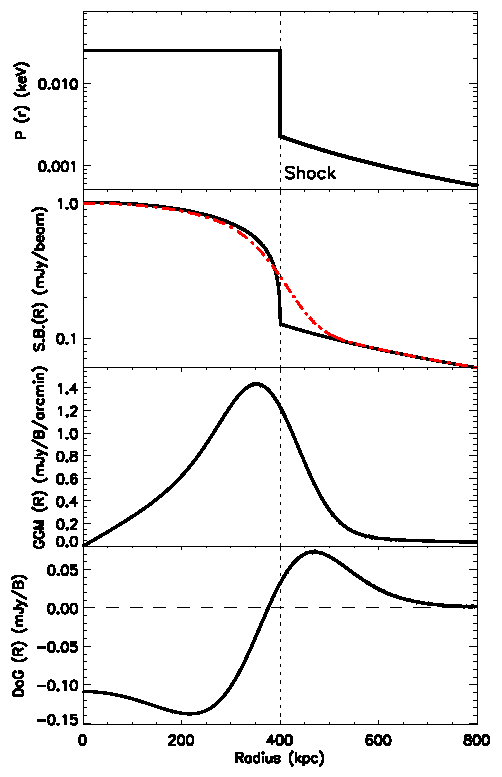
\includegraphics[trim=0cm 0cm 0cm 0cm, clip=true, width=0.49\textwidth]{Figure/Profiles_shock_15_15_45.pdf}
\caption{\footnotesize{GGM response to a shock propagating in a radially symmetrical way, with Mach number $\mathcal{M} = 3$. The black lines correspond to a shock propagating from core to outskirt, while the red dashed-dotted line correspond to the opposite case. The shock position is given by the vertical dashed line.
{\bf Top:} pressure profile as a function of the physical radius in 3D. 
{\bf Middle:} Compton parameter profile as a function of projected radius in 2D. 
{\bf Bottom:} GGM radial profile as a function of projected radius in 2D.}}
\label{fig:test_filter_shock}
\end{figure}



%###############################################################################################
%##########################                      Application to simulations                        ##########################
%###############################################################################################
\section{Application to hydrodynamical simulations}\label{sec:Application_to_hydrodynamical_simulations}
\begin{table*}[]
\caption{\footnotesize{Summary of the properties of the RHAPSODY-G selected cluster sample.}}
\begin{center}
%\resizebox{\textwidth}{!} {
\begin{tabular}{c|c|c|c|c|c}
\hline
\hline
Name & $z$ & kpc/arcsec & $M_{500}$ ($10^{14}$ M$_{\odot}$)& $Y_{500}$ ($10^{-3}$arcmin$^2$) & Comments \\
\hline
RG361\_00188 & 0.61 & 6.9 & 3.8 & 0.23 & Very relaxed, elongated along the line-of-sight \\ 
RG474\_00172 & 0.90 & 8.0 & 4.1 & 0.20 & Major merger after the first crossing of the two main cores \\ 
RG377\_00181 & 0.54 & 6.5 & 3.7 & 0.24 & Multiple merger \\
RG448\_00211 & 0.40 & 5.5 & 3.5 & 0.29 & Pressure shell caused by the central AGN \\ 
\hline
\end{tabular}
%}
\end{center}
\label{tab:rhapsody_summary}
\end{table*}

\begin{figure*}[h]
\resizebox{\textwidth}{!} {
\begin{tabular}{cccc}
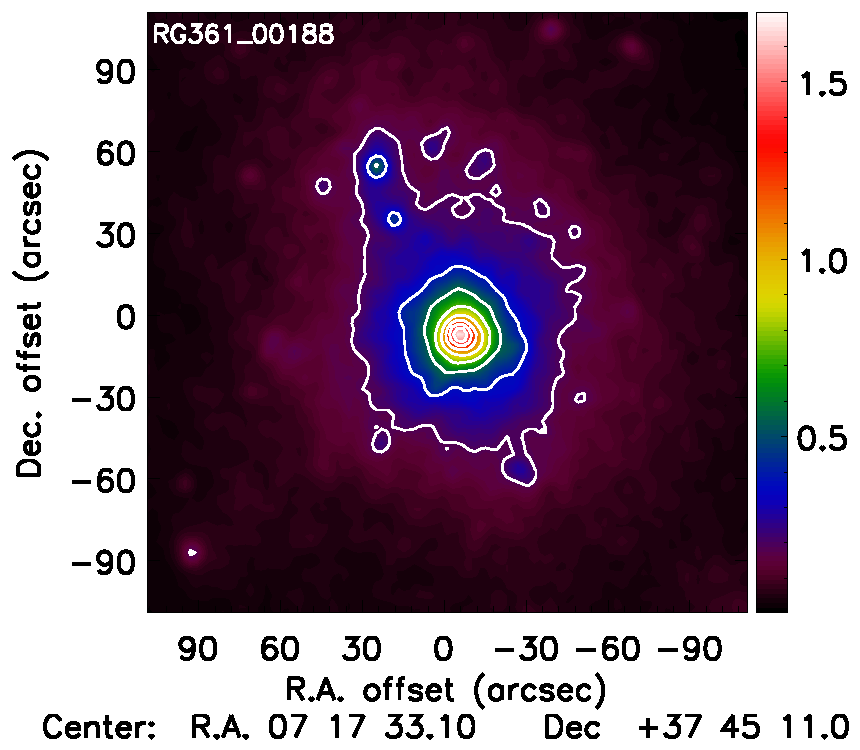
\includegraphics[trim=0cm 2.2cm 0cm 0cm, clip=true, scale=0.39]{Figure/Map_RG361_00188_DMmap_zproj_zobs0p6_raw.pdf} &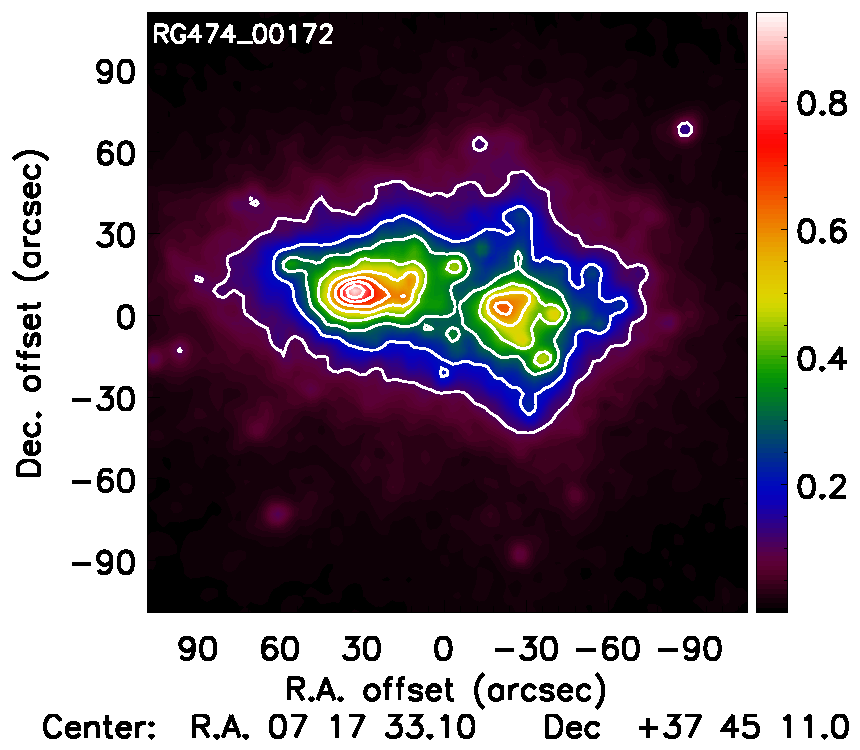
\includegraphics[trim=2.45cm 2.2cm 0cm 0cm, clip=true, scale=0.39]{Figure/Map_RG474_00172_DMmap_zproj_zobs0p9_raw.pdf} & 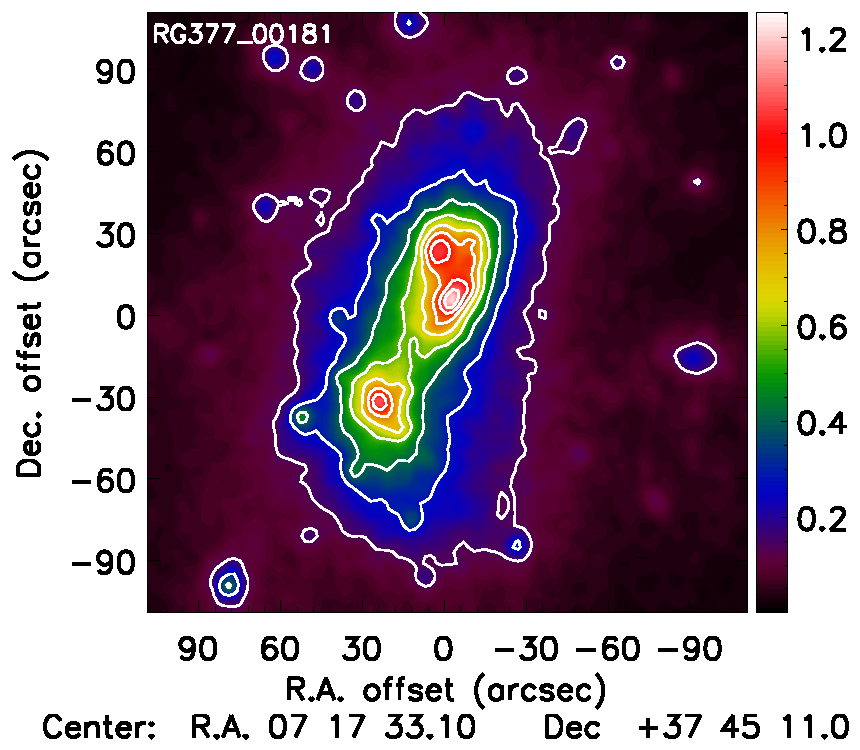
\includegraphics[trim=2.45cm 2.2cm 0cm 0cm, clip=true, scale=0.39]{Figure/Map_RG377_00181_DMmap_zproj_zobs0p5_raw.pdf} & 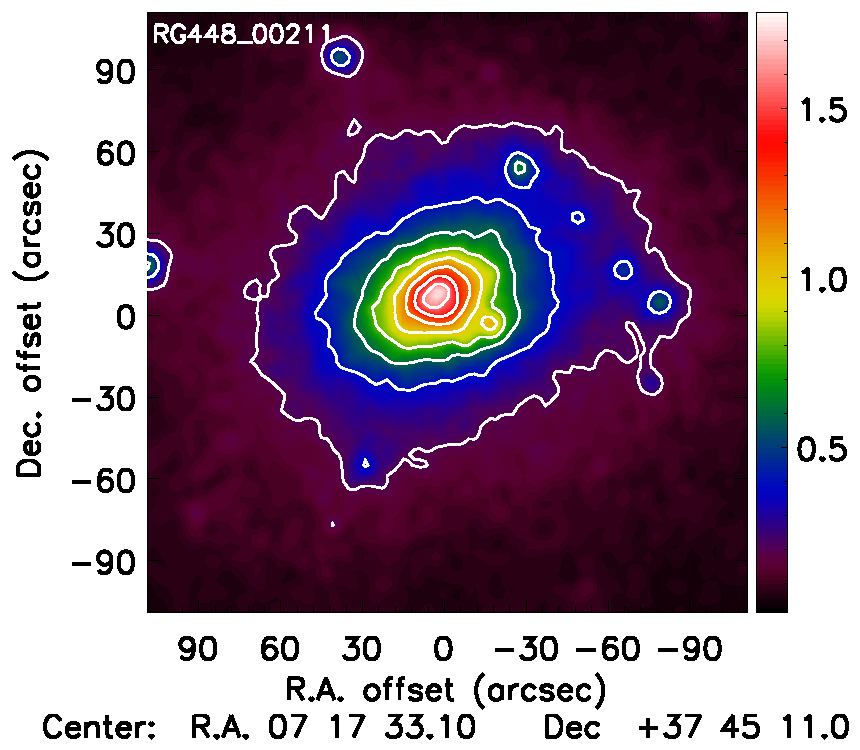
\includegraphics[trim=2.45cm 2.2cm 0cm 0cm, clip=true, scale=0.39]{Figure/Map_RG448_00211_DMmap_zproj_zobs0p4_raw.pdf} \\

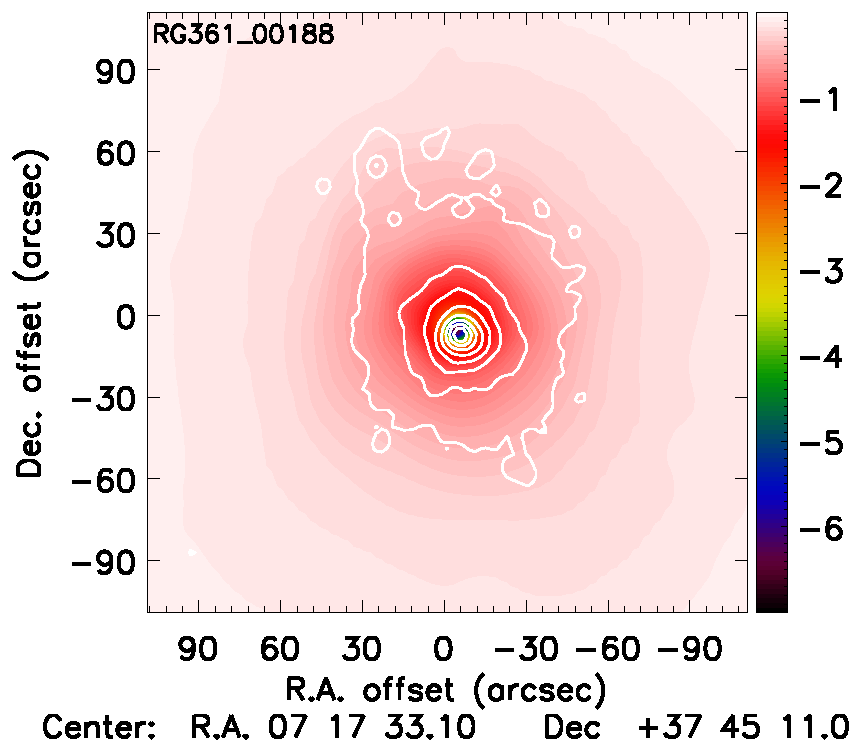
\includegraphics[trim=0cm 2.2cm 0cm 1.0cm, clip=true, scale=0.39]{Figure/Map_RG361_00188_Ymap_zobs0p6_raw.pdf} &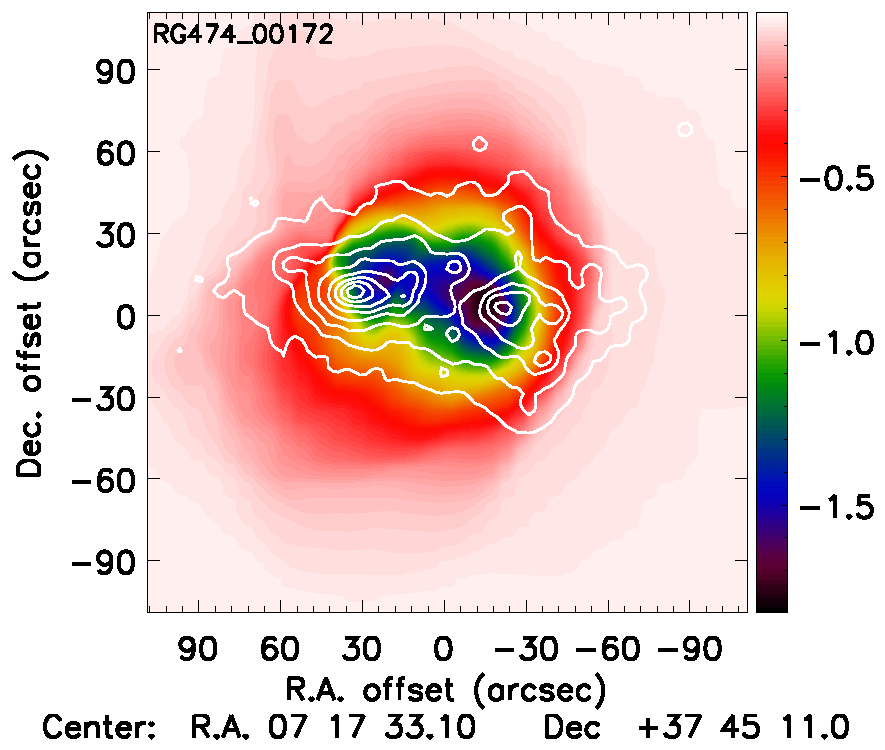
\includegraphics[trim=2.45cm 2.2cm 0cm 1.0cm, clip=true, scale=0.39]{Figure/Map_RG474_00172_Ymap_zobs0p9_raw.pdf} & 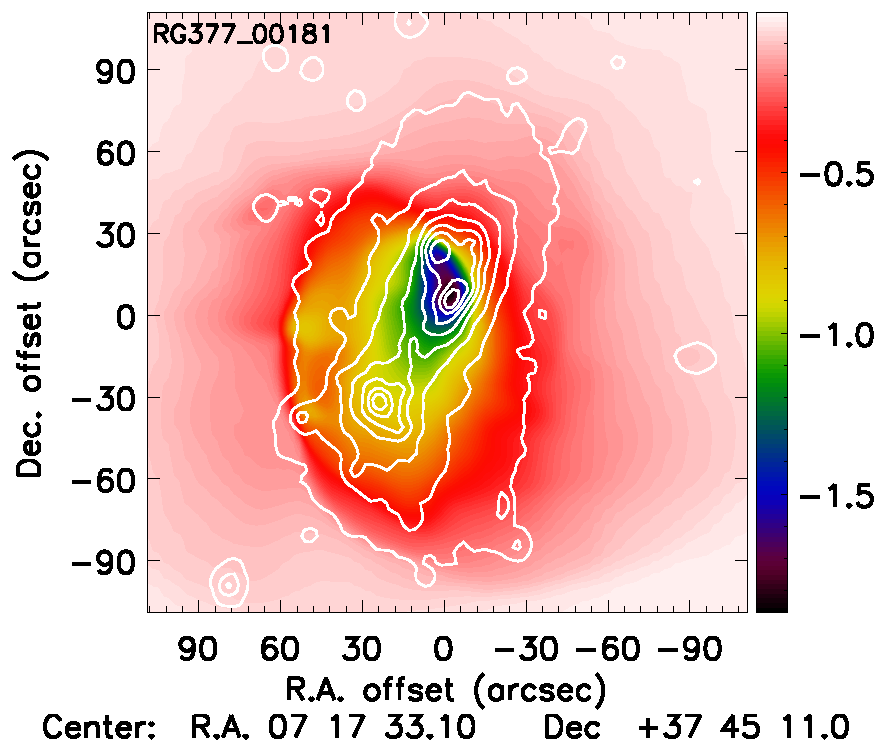
\includegraphics[trim=2.45cm 2.2cm 0cm 1.0cm, clip=true, scale=0.39]{Figure/Map_RG377_00181_Ymap_zobs0p5_raw.pdf} & 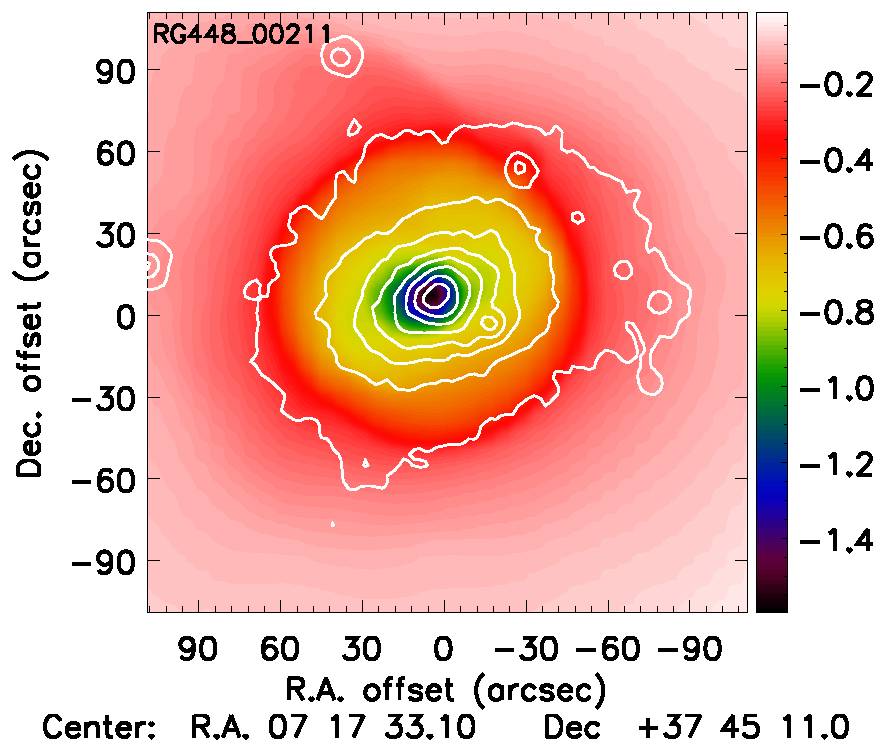
\includegraphics[trim=2.45cm 2.2cm 0cm 1.0cm, clip=true, scale=0.39]{Figure/Map_RG448_00211_Ymap_zobs0p4_raw.pdf} \\

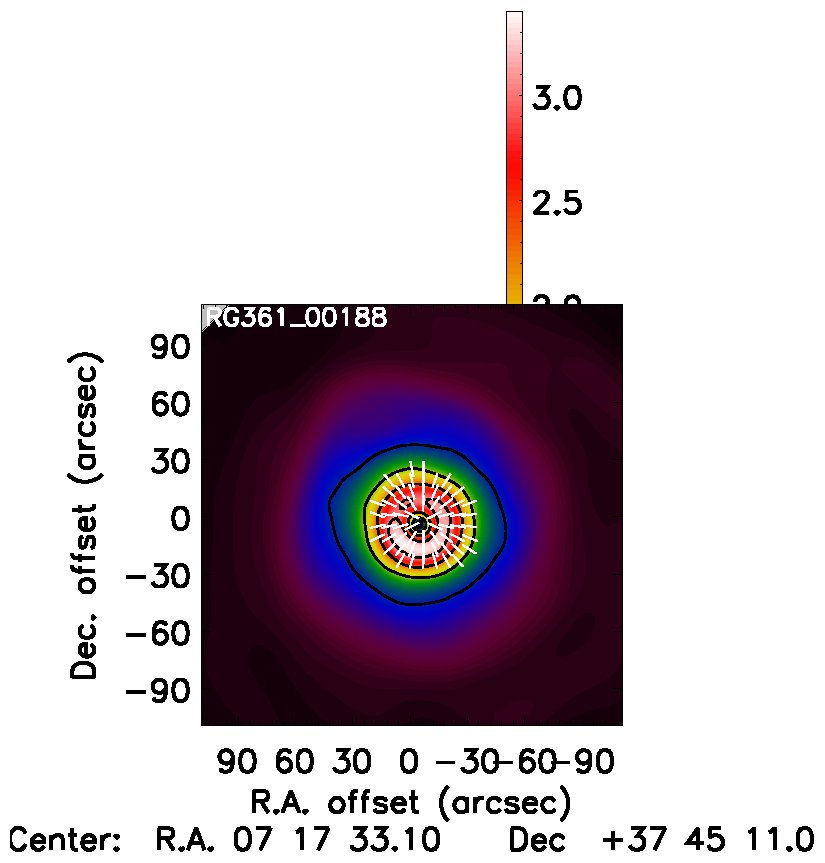
\includegraphics[trim=0cm 2.2cm 0cm 1.0cm, clip=true, scale=0.39]{Figure/Grad_RG361_00188_Ymap_zobs0p6_regrid_15_15_45.pdf} & 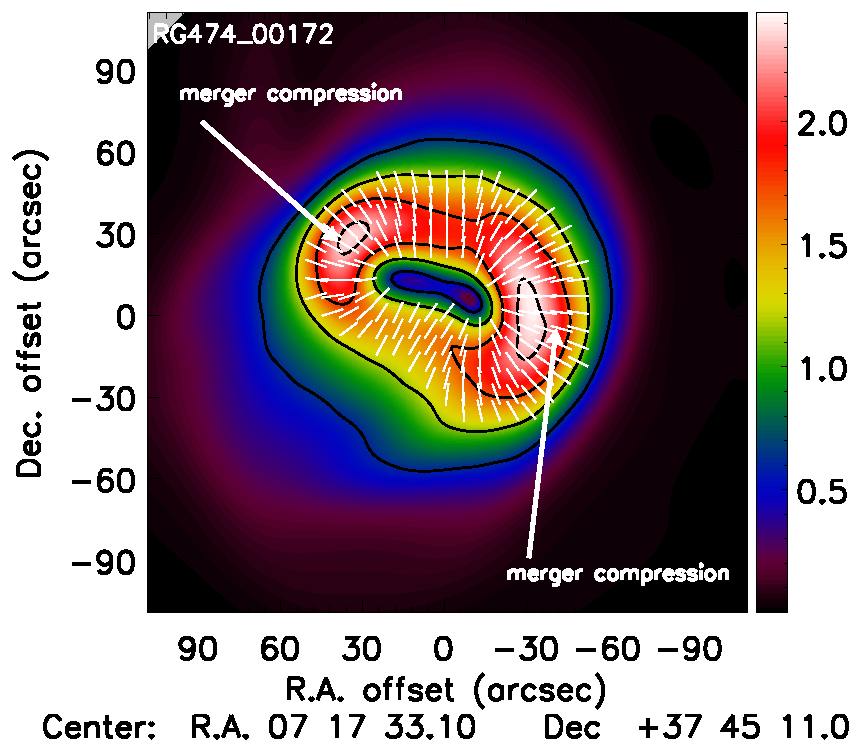
\includegraphics[trim=2.45cm 2.2cm 1.9cm 1.0cm, clip=true, scale=0.39]{Figure/Grad_RG474_00172_Ymap_zobs0p9_regrid_15_15_45.pdf} & 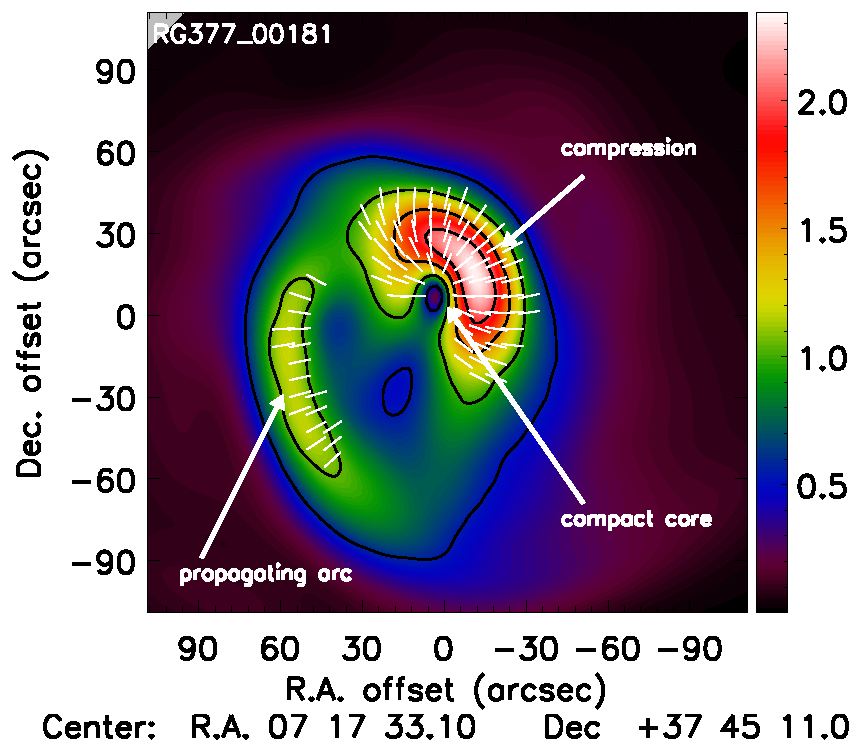
\includegraphics[trim=2.45cm 2.2cm 0cm 1.0cm, clip=true, scale=0.39]{Figure/Grad_RG377_00181_Ymap_zobs0p5_regrid_15_15_45.pdf} & 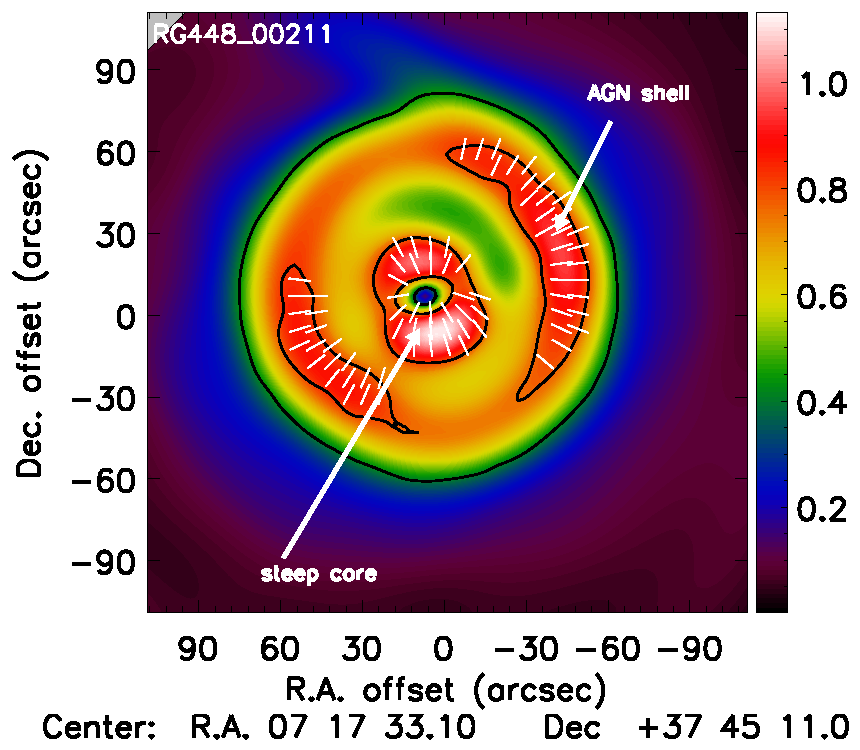
\includegraphics[trim=2.45cm 2.2cm 0cm 1.0cm, clip=true, scale=0.39]{Figure/Grad_RG448_00211_Ymap_zobs0p4_regrid_15_15_45.pdf} \\

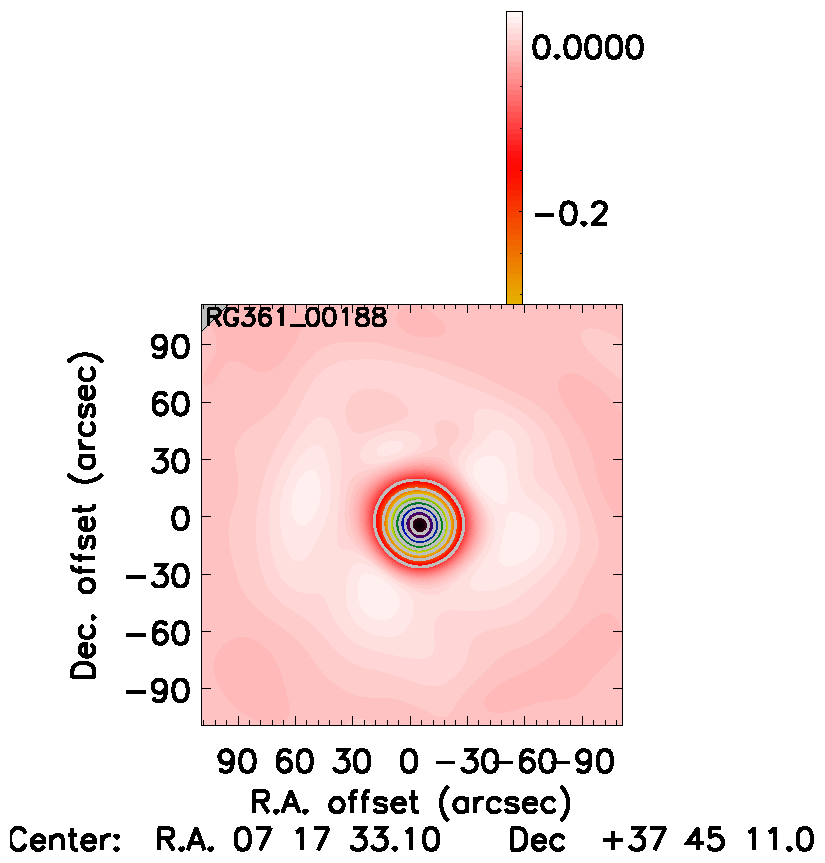
\includegraphics[trim=0cm 0.7cm 0.0cm 1.0cm, clip=true, scale=0.39]{Figure/DoG_RG361_00188_Ymap_zobs0p6_regrid_15_15_45.pdf} & 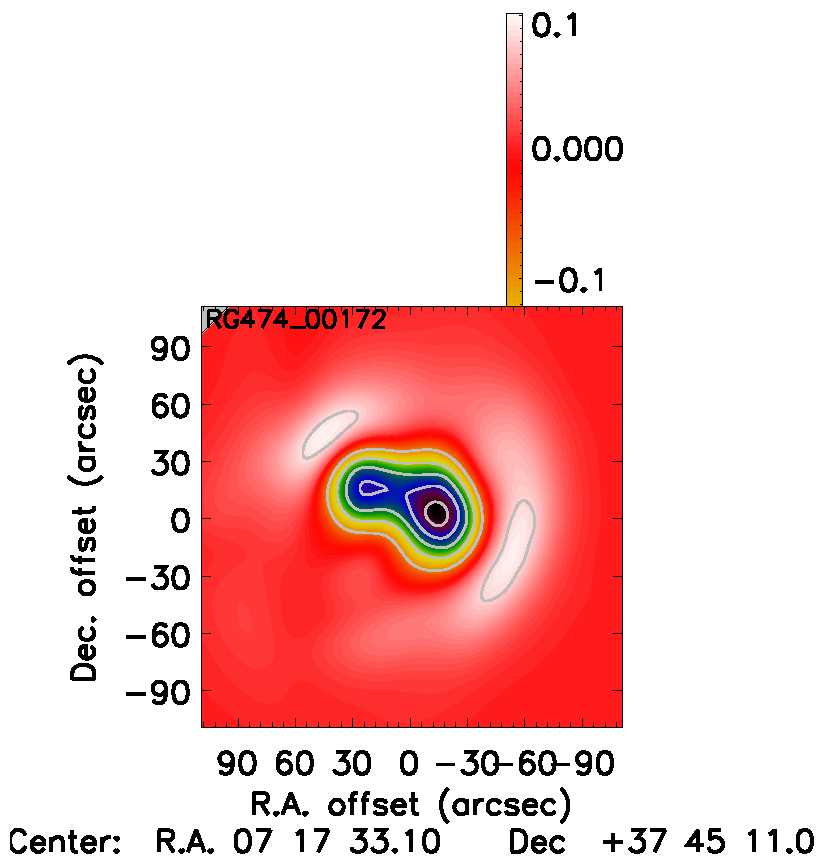
\includegraphics[trim=2.45cm 0.7cm 0.0cm 1.0cm, clip=true, scale=0.39]{Figure/DoG_RG474_00172_Ymap_zobs0p9_regrid_15_15_45.pdf} & 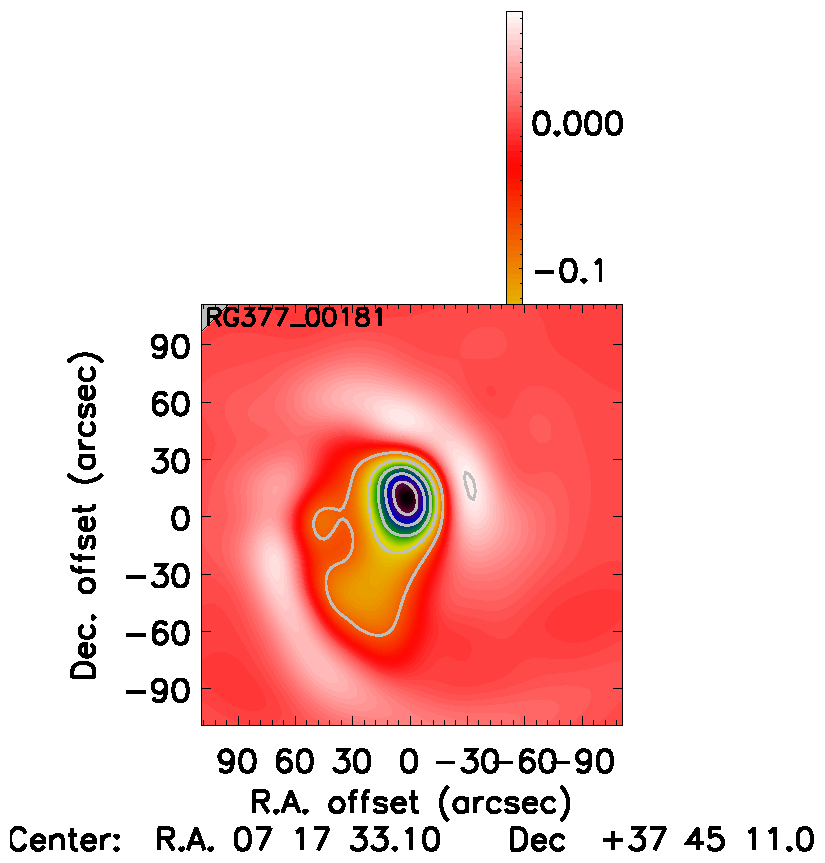
\includegraphics[trim=2.45cm 0.7cm 0.0cm 1.0cm, clip=true, scale=0.39]{Figure/DoG_RG377_00181_Ymap_zobs0p5_regrid_15_15_45.pdf} & 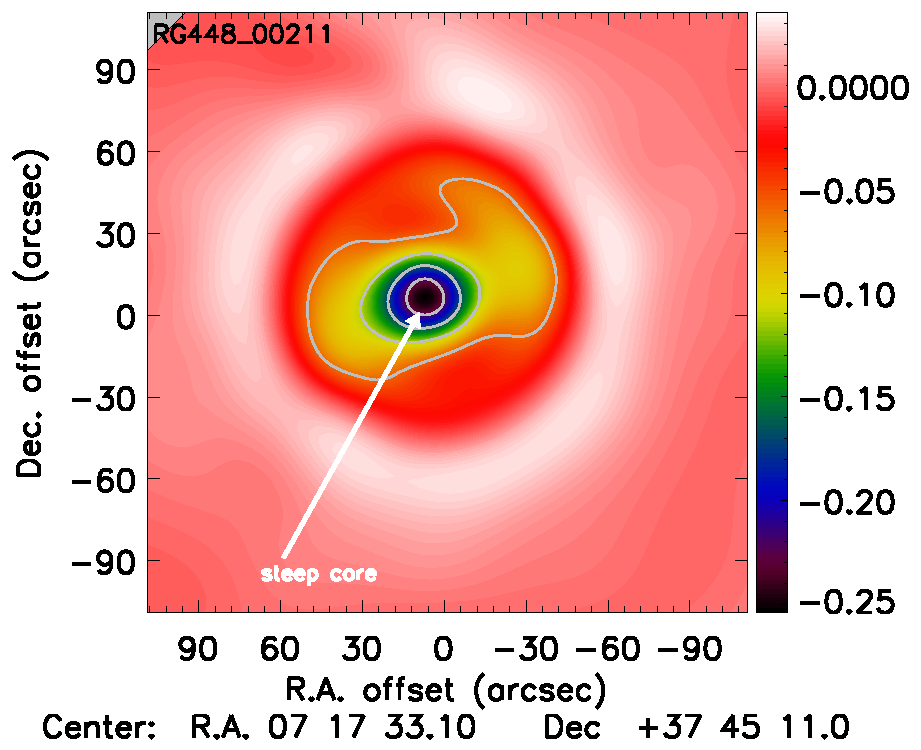
\includegraphics[trim=2.45cm 0.7cm 0.0cm 1.0cm, clip=true, scale=0.39]{Figure/DoG_RG448_00211_Ymap_zobs0p4_regrid_15_15_45.pdf}
\end{tabular}
}
\caption{\footnotesize{Application of the filtering algorithms to clusters from the RHAPSODY-G suite of simulations. From left to right, the clusters are RG361\_00188, RG474\_00172, RG377\_00181 and RG448\_00211 (see also Table \ref{tab:rhapsody_summary} for the main properties of the sample). {\bf First row:} projected dark matter density. Contours are linearly spaced. Units are arbitrary. {\bf Second row:} input raw surface brightness maps with dark matter map contours overlaid. Units are mJy/beam. {\bf Third row:} GGM filtered maps with $\theta_0 = 15"$. The white vectors represent the direction of the gradient, $\Psi$. Units are mJy/beam/arcmin. {\bf Bottom row:} DoG filtered maps with $\theta_1 = 15"$ and $\theta_2 = 45"$. Units are mJy/beam. The contours provide the true signal-to-noise expected for the simulation of the observation of these sources done in section \ref{sec:Systematics_and_noise_properties}. They are given by steps of $2 \sigma$ excluding 0 (see section \ref{sec:Systematics_and_noise_properties} for further discussions about the signal-to-noise estimates).}}
\label{fig:RG_cluster_sample}
\end{figure*}

Before performing our analysis on the NIKA data, we test the behavior of the filters described in section \ref{sec:Pressure_substructures_detection} by using realistic simulated cluster data. Such simulations also aid in the interpretation of the observed structures in real data. To do so, we use synthetic tSZ images extracted from the RHAPSODY-G simulations for different cluster configurations.

%==================== Simulations
\subsection{Extraction of tSZ maps from the RHAPSODY-G simulations}
The RHAPSODY-G simulations \citep{Wu2013,Hahn2017} is a suite of cosmological hydrodynamics adaptive mesh refinement zoom simulations of ten massive clusters. The simulations include cooling and sub-resolution models for star formation and supermassive black hole feedback. 

Boxes of co-moving volume $\left(5 \ {\rm Mpc}\right)^3$ were used to extract Compton parameter maps around the clusters by integrating equation \ref{eq:y_compton} along a fixed line-of-sight direction, using the gas pressure in each grid cell. These maps were converted into surface brightness images, in the NIKA 150 GHz bandpasses \citep[see the coefficient provided in][]{Adam2016b}. We neglect relativistic corrections, as they can only reduce the surface brightness by up to 8\% for the hottest clusters at our frequency \citep{Itoh2003}. The maps were produced for a large subset of the available simulation snapshots (about 150 per cluster), tracing the evolution of the clusters from redshift $z \sim 1.5$ to $z=0$. The knowledge of the clusters formation history is a key point for the interpretation of the maps.

%==================== Selection
\subsection{Selection of a RHAPSODY-G sub-sample}\label{sec:Selection_of_a_RHAPSODY-G_sub-sample}
A sub-sample of clusters was selected to assess the sub-structure detection in a quantitative way and to investigate the behavior of the filters in details (see section \ref{sec:Systematics_and_noise_properties} for the end-to-end processing of the simulations). The clusters were selected to match the redshift range of the NIKA sample (see section \ref{sec:NIKA_Data}) and to explore various cluster configurations. We thus restricted the RHAPSODY-G snapshots to the redshift range $0.4<z<1$ and selected four distinct snapshots, by visual inspection, for different clusters:
\begin{enumerate}
\item {\bf RG361\_00188:} a relaxed spherical cluster at redshift $z = 0.61$, with minimal merging activity since $z \gtrsim 1$. The cluster is slightly elongated along the line-of-sight.
\item {\bf RG474\_00172:} a major merger at $z = 0.90$. The two main sub-clusters already passed trough each other, the closest encounter happening at $z \sim 0.95$. The merger axis is close to be in the plane of the sky. 
\item {\bf RG377\_00181:} a triple-merger with two nearly equal mass objects and a smaller sub-group at $z = 0.54$. The two main sub-clusters have already experienced the first encounter at $z \sim 0.59$, while the smaller group is coincident with one of the two main clusters.
\item {\bf RG448\_00211:} a relaxed, slightly elliptical cluster, exhibiting strong AGN feedback at $z = 0.40$. This produces a pressure shell around the main core.
\end{enumerate}
We note that the RHAPSODY-G cluster masses match well those of the NIKA sample at redshift zero, but they are lower by a factor of a few at the considered redshifts. Therefore the simulated surface brightnesses are also lower by a factor of $\sim 2$. The summary of the main properties of the four RHAPSODY-G selected clusters is provided in table \ref{tab:rhapsody_summary}.

%==================== Filter
\subsection{Filter application to raw RHAPSODY-G tSZ images}
We first apply the filters defined in section \ref{sec:Pressure_substructures_detection} to the raw RHAPSODY-G surface brightness images (i.e. without including noise or observation artifacts). The filtering parameters are set according to our baseline choice (section \ref{sec:Baseline_filtering_parameters}), as optimized for the NIKA sample. Figure \ref{fig:RG_cluster_sample} provides images of the input surface brightness of the RHAPSODY-G selected sample, and the corresponding filtered maps together with the projected dark matter density distribution. 

RG361\_00188 (relaxed) presents a very compact core and is azimuthally symmetric. The tSZ signal matches well that of the dark matter. As the steepness of the surface brightness profile increases toward the center, the corresponding GGM map is null at the cluster peak and exhibit a quasi perfect ring of radius matched to the filter scale, with a small excess in the south. The DoG map presents a single compact core component. The RG474\_00172 and RG377\_00181 (major and multiple mergers, respectively) tSZ maps show that the two clusters are both clearly disturbed. The corresponding dark matter maps reflect the presence of multiple sub-clusters and the dark matter distribution deviates significantly from that of the tSZ signal. The GGM maps provide additional information by highlighting regions of strong gas compression. In the case of the major merger, RG474\_00172, we observe a strongly elongated ring with two main pressure gradients in the east and west regions. In the case of the multiple merger, RG377\_00181, a strong gradient is visible in the west region, corresponding to the main core, and a $\sim 70$ arcsec (460 kpc) long arc propagates through the ICM on the southeast sector, corresponding to another sub-cluster moving within the ICM of the main cluster. The DoG maps present a double peak structure, allowing us to quantitatively identify the two subclusters in the case of RG474\_00172. On the other hand, one only finds a main core plus a weak extension in the case of RG377\_00181. RG448\_00211 appears to be relatively relaxed and azimuthally symmetric, in agreement with the dark matter distribution. However, the GGM map reveals, in addition to the steep core, the presence of a pressure shell responsible for a strong gradient ring extending 45 arcsec (250 kpc) away from the peak. This is due to the feedback from the central AGN onto the ICM, and possibly an artifact of the specific implementation of AGN feedback as a thermal blastwave in these simulations. We also observe a plateau extending to 45 arcsec (250 kpc) radius on the DoG filtered map and we note that the core signal is slightly elongated with a main axis inclined about 20 degrees with respect to the R.A. axis.

The morphologies seen in the filtered RHAPSODY-G sub-sample thus provide templates that we can compare to the structures observed in the real NIKA data. In practice, we performed this analysis using all available RHAPSODY-G snapshots and projected the data along three line-of-sight directions. Therefore, we dispose of a much larger variety of configurations, even if the four selected clusters already sample most of the structures visible in the simulation, according to the selection of the sub-sample. These templates will allow us to better understand the physics at play in the NIKA clusters, in particular in merging systems. When using the tSZ signal as a tracer of the overall matter distribution \citep[e.g.][]{Adam2015,Adam2016a,Ruppin2016}, the application of such filters could also help interpreting scatters and biases between the total mass distribution and the tSZ signal, as such features reflect spatial misalignment between the dark matter distribution and the hot gas.

In summary, the GGM and the DoG filters allow us to identify gas compression regions and sub-groups in the RHAPSODY-G images, respectively. They provide templates for interpreting features observed in the NIKA data in section \ref{sec:Application_to_the_NIKA_clusters_sample}.

%###############################################################################################
%##########################                        Systematics and noise                          ##########################
%###############################################################################################
\section{Systematic effects and noise properties}\label{sec:Systematics_and_noise_properties}
In addition to the tSZ sub-structures, NIKA data are affected by several systematic effects that can potentially alter the reconstructed filtered images. In this section we test the response of the filters described in section \ref{sec:Pressure_substructures_detection} to potential bouncing artifacts due to the transfer function of the NIKA processing, spatially correlated noise, and point source residuals.

\begin{figure*}[h]
\resizebox{\textwidth}{!} {
\begin{tabular}{cccc}
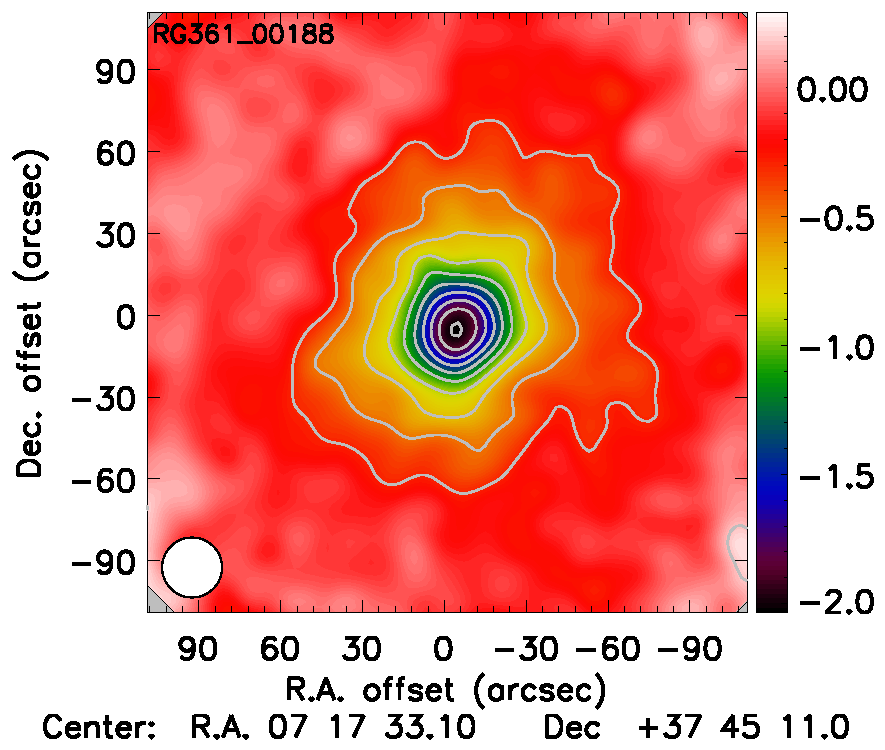
\includegraphics[trim=0cm 2.2cm 0cm 0cm, clip=true, scale=0.39]{Figure/Map_RG361_00188_Ymap_zobs0p6_processed.pdf} &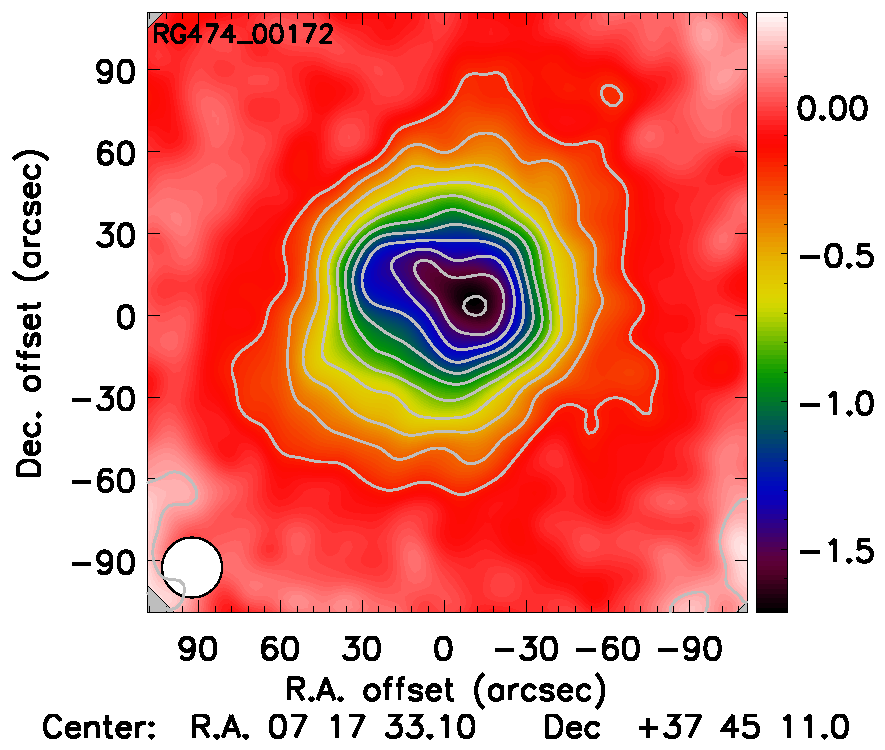
\includegraphics[trim=2.45cm 2.2cm 0cm 0cm, clip=true, scale=0.39]{Figure/Map_RG474_00172_Ymap_zobs0p9_processed.pdf} &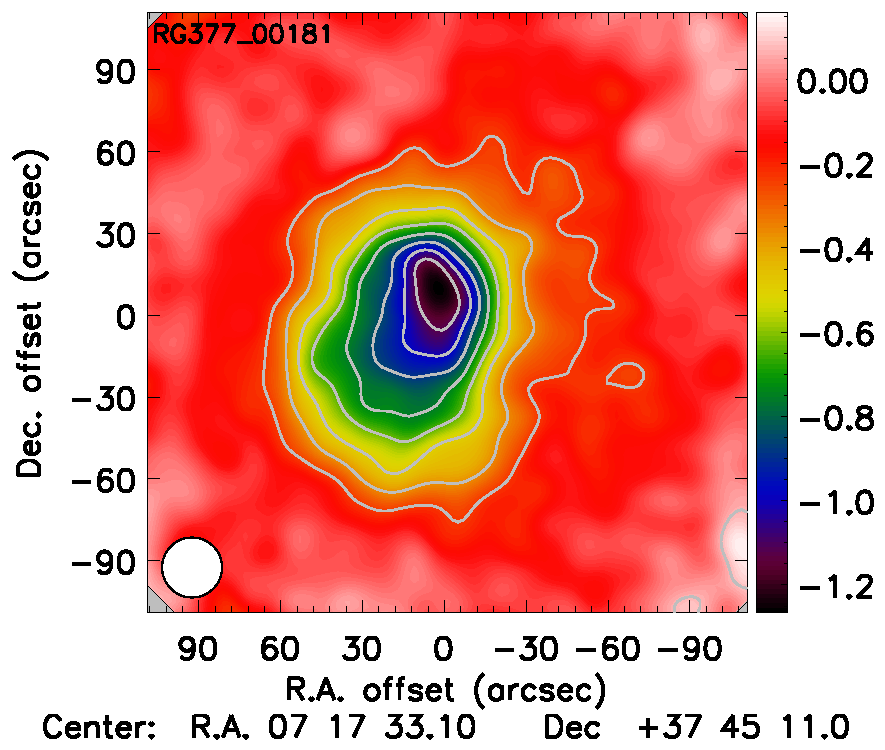
\includegraphics[trim=2.45cm 2.2cm 0cm 0cm, clip=true, scale=0.39]{Figure/Map_RG377_00181_Ymap_zobs0p5_processed.pdf} &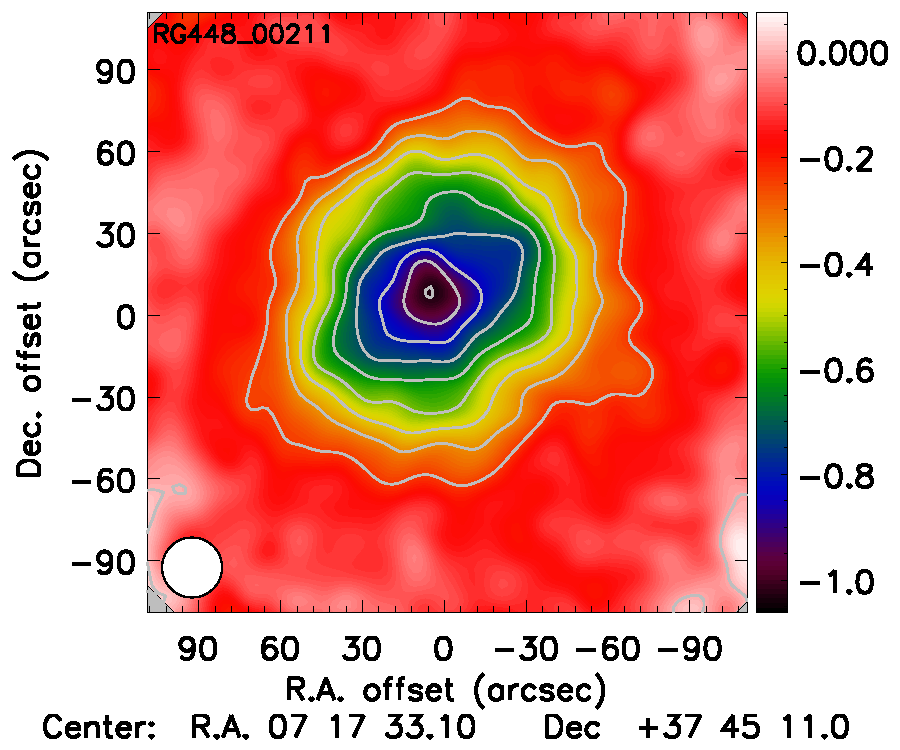
\includegraphics[trim=2.45cm 2.2cm 0cm 0cm, clip=true, scale=0.39]{Figure/Map_RG448_00211_Ymap_zobs0p4_processed.pdf} \\

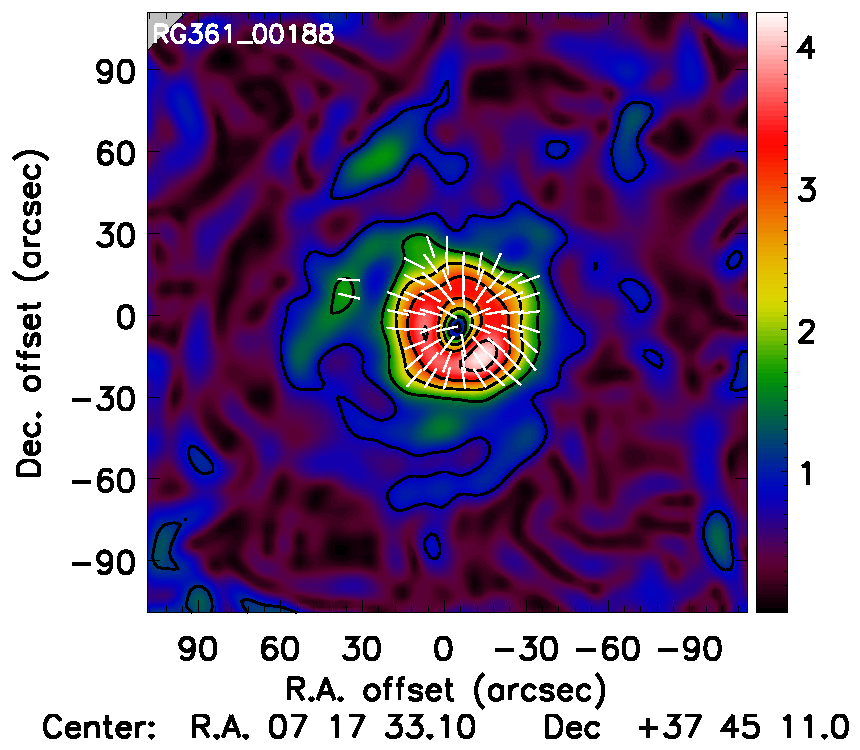
\includegraphics[trim=0cm 2.2cm 0cm 0cm, clip=true, scale=0.39]{Figure/Grad_RG361_00188_Ymap_zobs0p6_processed_15_15_45.pdf} & 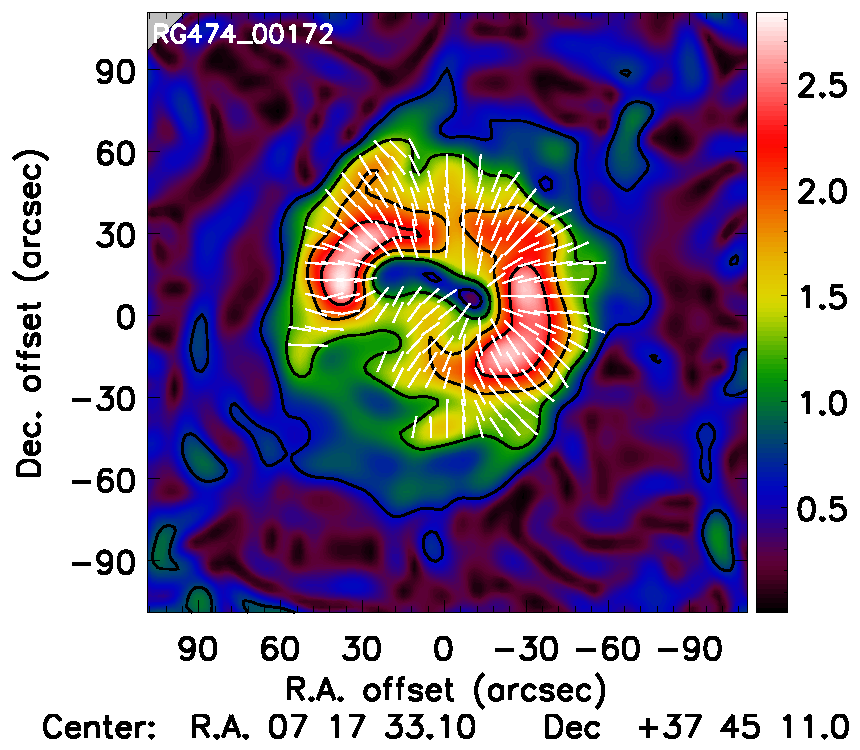
\includegraphics[trim=2.45cm 2.2cm 0cm 0cm, clip=true, scale=0.39]{Figure/Grad_RG474_00172_Ymap_zobs0p9_processed_15_15_45.pdf} & 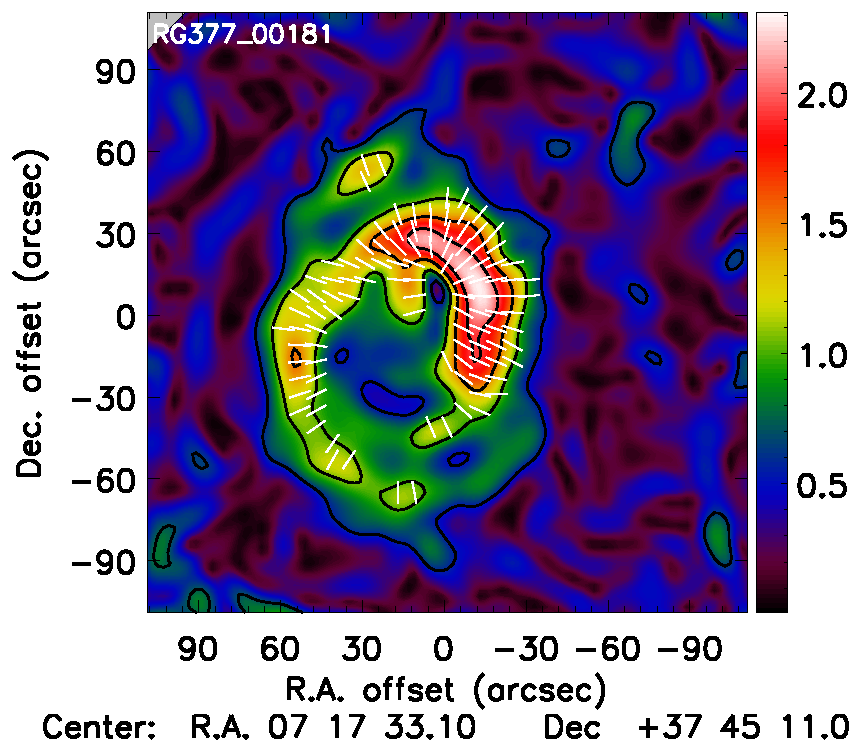
\includegraphics[trim=2.45cm 2.2cm 0cm 0cm, clip=true, scale=0.39]{Figure/Grad_RG377_00181_Ymap_zobs0p5_processed_15_15_45.pdf} & 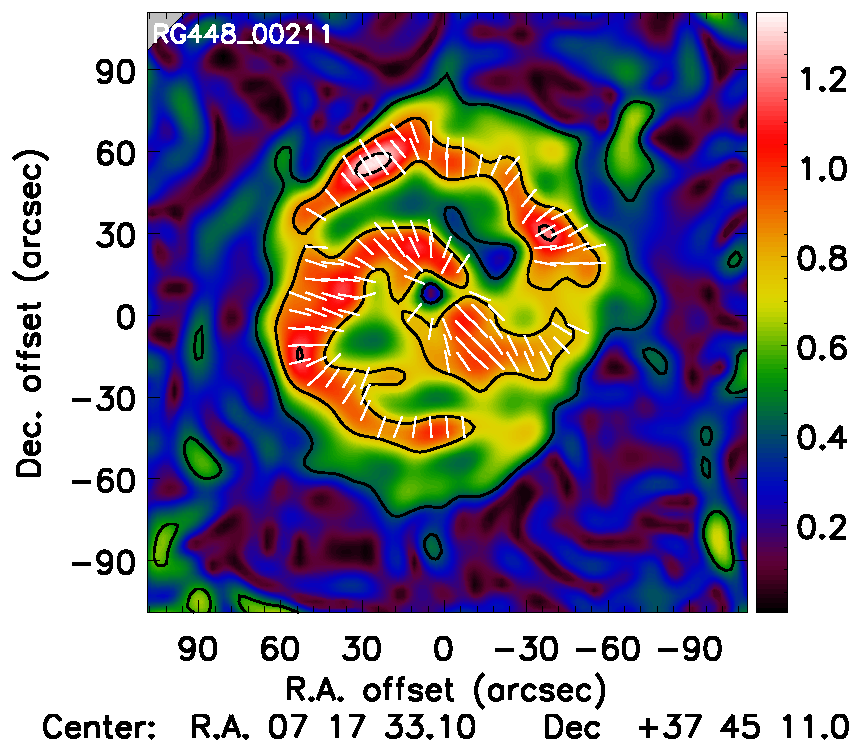
\includegraphics[trim=2.45cm 2.2cm 0cm 0cm, clip=true, scale=0.39]{Figure/Grad_RG448_00211_Ymap_zobs0p4_processed_15_15_45.pdf} \\

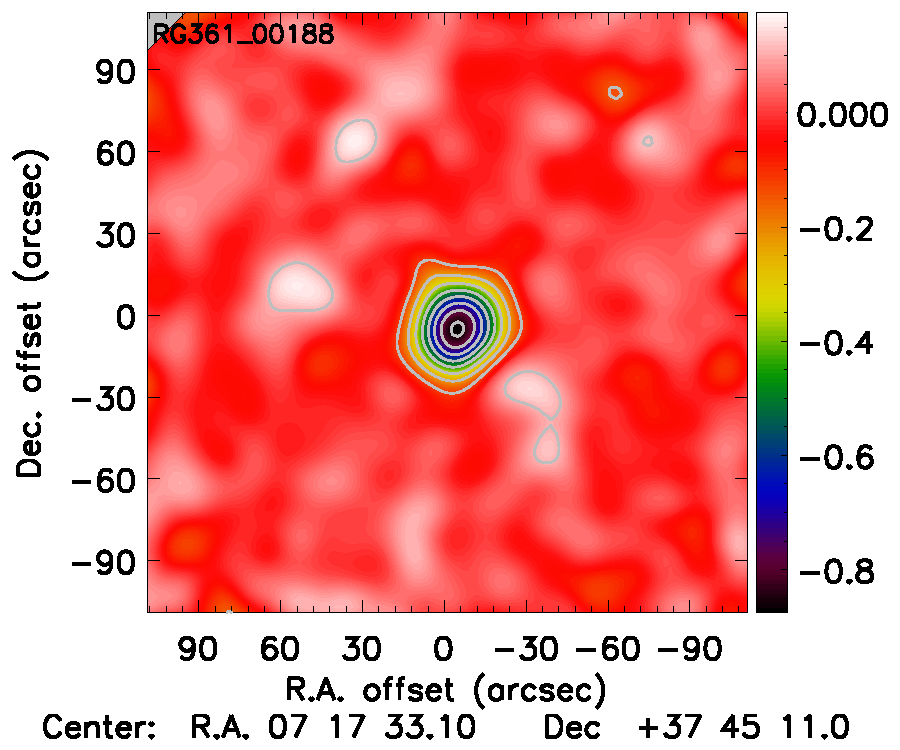
\includegraphics[trim=0cm 0.7cm 0cm 0cm, clip=true, scale=0.39]{Figure/DoG_RG361_00188_Ymap_zobs0p6_processed_15_15_45.pdf} & 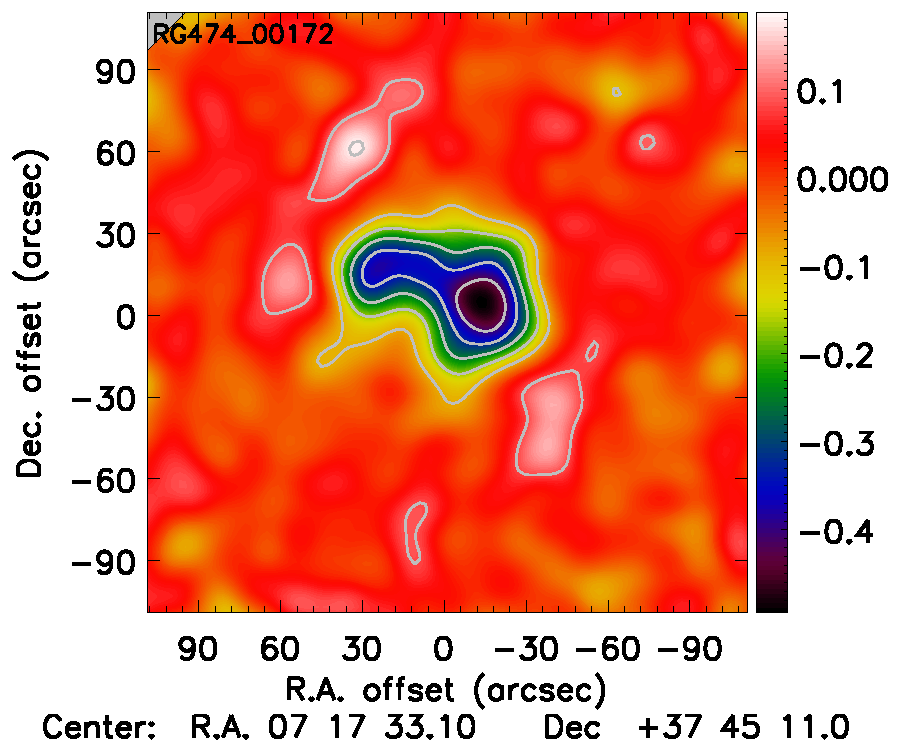
\includegraphics[trim=2.45cm 0.7cm 0cm 0cm, clip=true, scale=0.39]{Figure/DoG_RG474_00172_Ymap_zobs0p9_processed_15_15_45.pdf} & 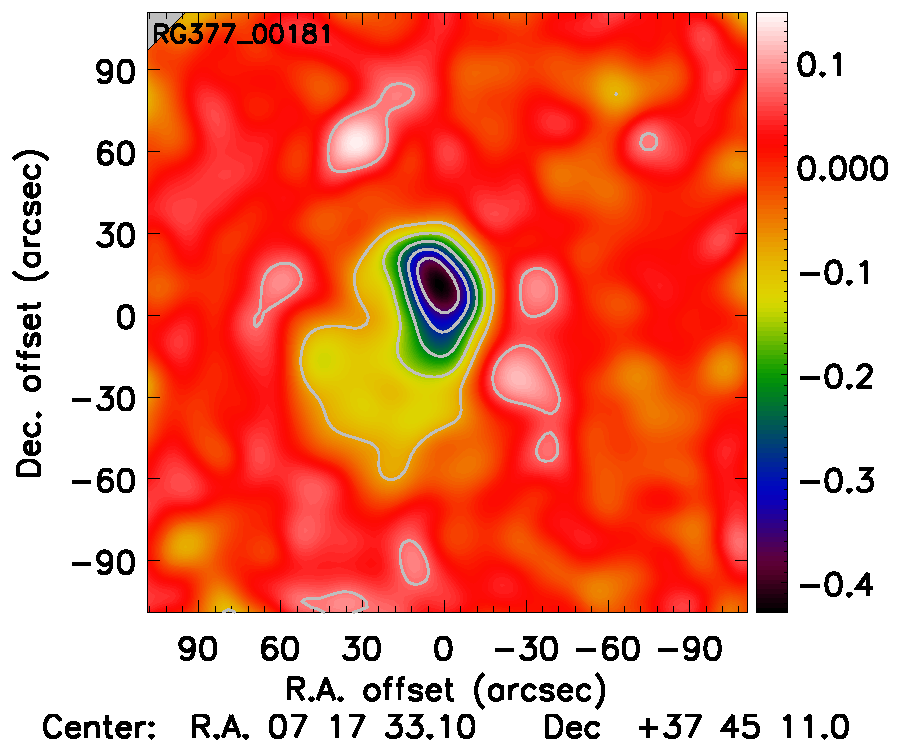
\includegraphics[trim=2.45cm 0.7cm 0cm 0cm, clip=true, scale=0.39]{Figure/DoG_RG377_00181_Ymap_zobs0p5_processed_15_15_45.pdf} & 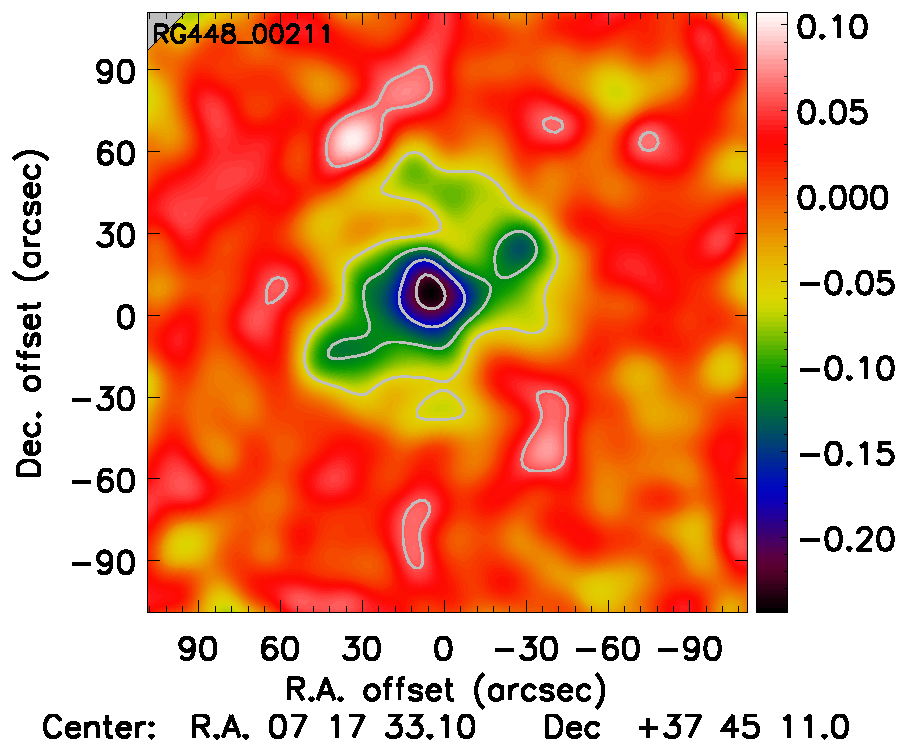
\includegraphics[trim=2.45cm 0.7cm 0cm 0cm, clip=true, scale=0.39]{Figure/DoG_RG448_00211_Ymap_zobs0p4_processed_15_15_45.pdf}
\end{tabular}
}
\caption{\footnotesize{Same as figure \ref{fig:RG_cluster_sample} in the case of end-to-end processing of the simulated RHAPSODY-G sub-sample: surface brightness maps (top), GGM filtered maps (middle) and DoG filtered maps (bottom). From left to right, the clusters are RG361\_00188, RG474\_00172, RG377\_00181 and RG448\_00211 (see also Table \ref{tab:rhapsody_summary} for the main properties of the sample). The surface brightness images are deconvolved from the transfer function (but not from the beam smoothing) and the signal-to-noise contours are estimated as in the case of real data (separated by steps of $2 \sigma$).}}
\label{fig:RG_cluster_sample_proc}
\end{figure*}

%==================== End to end processing of the RHAPSODY-G clusters
\subsection{NIKA processing of the RHAPSODY-G sub-sample}
While the DoG filter is linear and preserves the gaussian nature of the noise, this is not the case for the GGM filter. Therefore, in order to validate the behavior of the filter, we use end-to-end realistic simulations of the observations and post-processing of the RHAPSODY-G sub-sample, including all the artifacts present in the real data, but for which the true input signal is known.

To obtain simulated observed surface brightness images, we make use of the real raw telescope time ordered data (TOD) collected for the cluster \mbox{MACS~J0717.5+3745} (the one with the largest observing time, see section \ref{sec:Application_to_the_NIKA_clusters_sample}), in which we inject the signal corresponding to the considered RHAPSODY-G tSZ maps, according to the telescope scanning strategy. Prior adding the simulated signal to the data, half of the TOD scans are multiplied by $-1$ in order to cancel the astrophysical signal present in the real data, on the final co-added map. We aim at obtaining simulations corresponding to the highest signal-to-noise NIKA clusters. Therefore, before adding the simulated signal to the TOD, the noise is rescaled by the ratio of the RHAPSODY-G clusters peak surface brightness to the one of the deconvolved map of \mbox{MACS~J0717.5+3745} (typically a factor of $\sim 2$, see section \ref{sec:Selection_of_a_RHAPSODY-G_sub-sample}). The TOD are then processed similarly to the one of the real NIKA clusters \citep[see][for more details]{Adam2015}. 

Finally, we obtain realistic maps of the RHAPSODY-G sub-sample, as if they were truly observed using NIKA, with a signal-to-noise peak of about 20, at 22~arcsec resolution. The maps, once deconvolved from the processing transfer function (see section \ref{sec:Transfer_function_filtering}), are displayed in Figure~\ref{fig:RG_cluster_sample_proc}, together with their GGM and DoG filtered maps obtained using our baseline parameter values (cf. Section~\ref{sec:Baseline_filtering_parameters}). These maps can be compared to that of Figure~\ref{fig:RG_cluster_sample} to validate our procedure, and they are used in the following sub-sections to quantify the properties of the filtered maps in the presence of systematic effects and noise.

%==================== Transfer function
\subsection{Transfer function filtering}\label{sec:Transfer_function_filtering}
The reduction of the raw NIKA data affects the reconstructed astrophysical sky signal by filtering out structures on large scales. We compute the angular transfer function of the reduction, as described in \cite{Adam2015} and use it to deconvolve the data to compensate for filtering effects. The absolute zero level of the brightness on the map remains unconstrained when observing clusters with NIKA, and it cannot be corrected using the transfer function of the processing. This corresponds to the transfer function being zero at angular wavenumber $k = 0$. However, this does not affect the result presented in this paper since both the GGM and DoG filtering procedures are insensitive to zero level effects. After deconvolution, small differences can remain between the deconvolved image and the original input image, due in particular to anisotropies in the scanning strategy and uncertainties in the estimated transfer function. However, these differences are mostly prominent on scales larger than the NIKA field of view ($\sim 2$ arcmin), where filtering effect are important \citep{Adam2015}. By comparing the NIKA-like processed RHAPSODY-G sub-sample to the non-processed maps, we find that these differences have a negligible impact on the filter application with respect to the noise (see the bottom panels of figures \ref{fig:RG_cluster_sample} and \ref{fig:RG_cluster_sample_proc}).

%==================== Noise
\subsection{Noise spatial correlations and propagation through the filters}
\begin{figure*}[h]
\centering
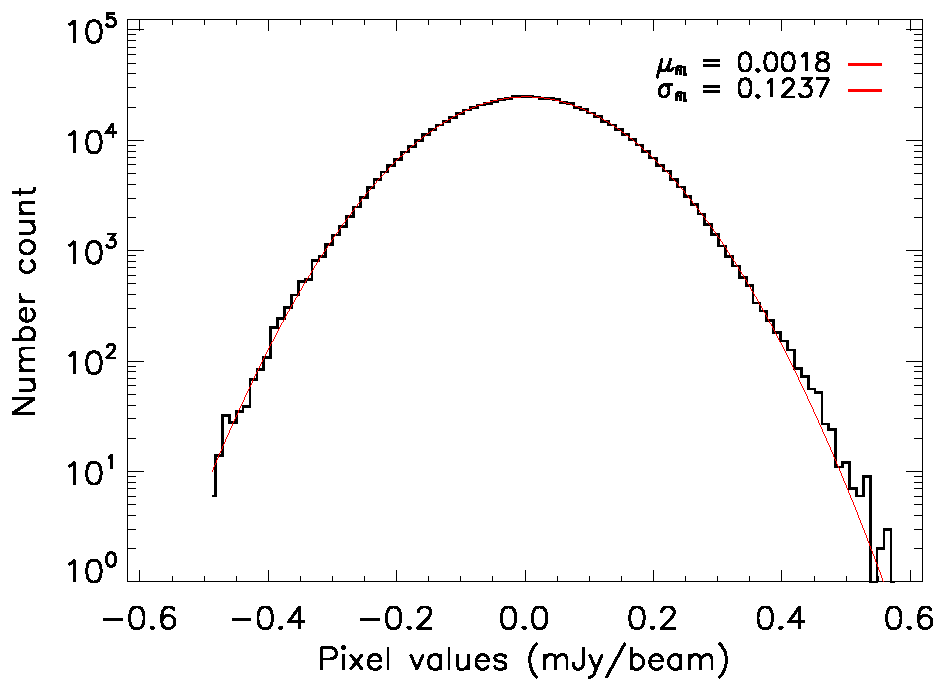
\includegraphics[trim=0cm 0cm 0cm 0cm, clip=true, totalheight=4.2cm]{Figure/DoG_noise_stat_CLJ1227.pdf}
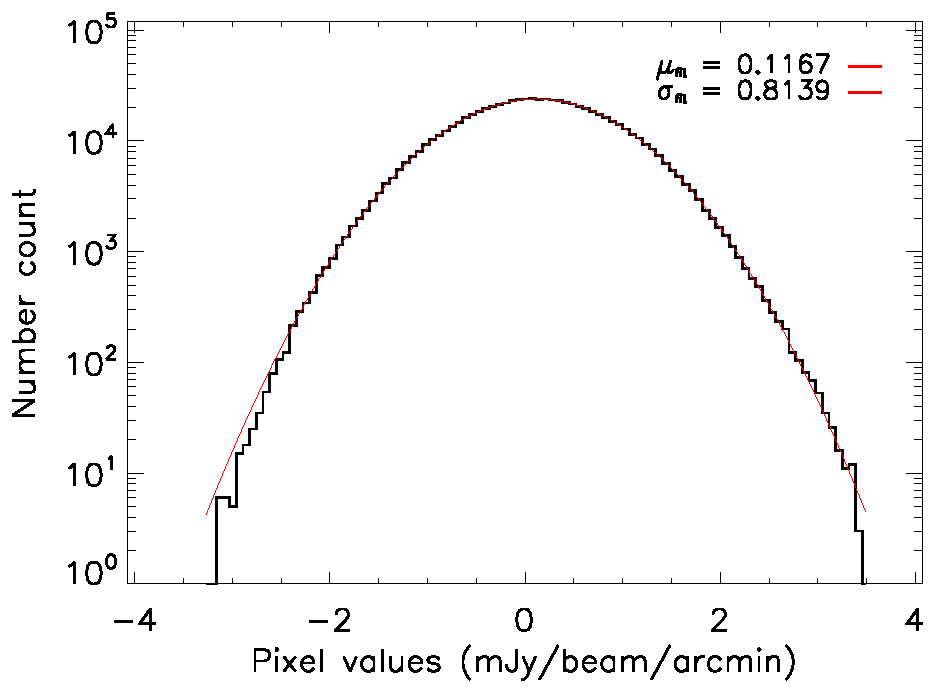
\includegraphics[trim=0cm 0cm 0cm 0cm, clip=true, totalheight=4.2cm]{Figure/GGM_noise_stat_CLJ1227.pdf}
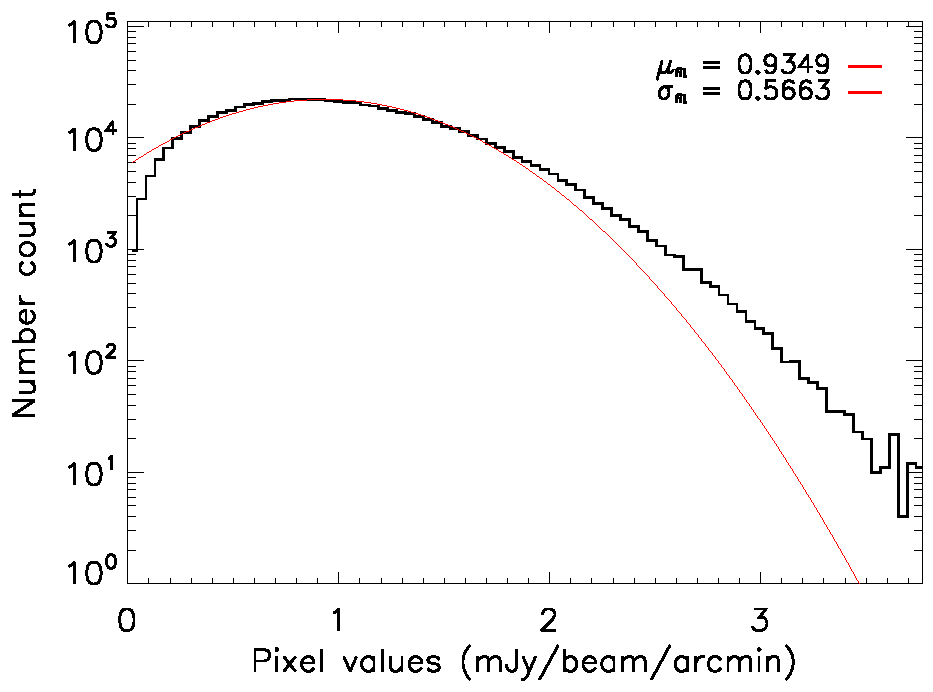
\includegraphics[trim=0cm 0cm 0cm 0cm, clip=true, totalheight=4.2cm]{Figure/GGM_noise_stat_CLJ1227_NoSignal.pdf}
\caption{\footnotesize{Noise distribution of all the pixels enclosed within 30 arcsec radius from the cluster center, in the case of \mbox{CL~J1226.9+3332}, for our baseline filter parameters. The red curves provides the best Gaussian fit to the histograms. {\bf Left:} DoG noise histogram. {\bf Middle:} GGM noise histogram in the case of $\hat{S}$ set to the observed signal of \mbox{CL~J1226.9+3332}. {\bf Right:} GGM noise histogram in the case where $\hat{S} = 0$ in equation \ref{eq:GGM_filter_noise}.}}
\label{fig:noise_statistics1}
\end{figure*}

\begin{figure}[h]
\centering
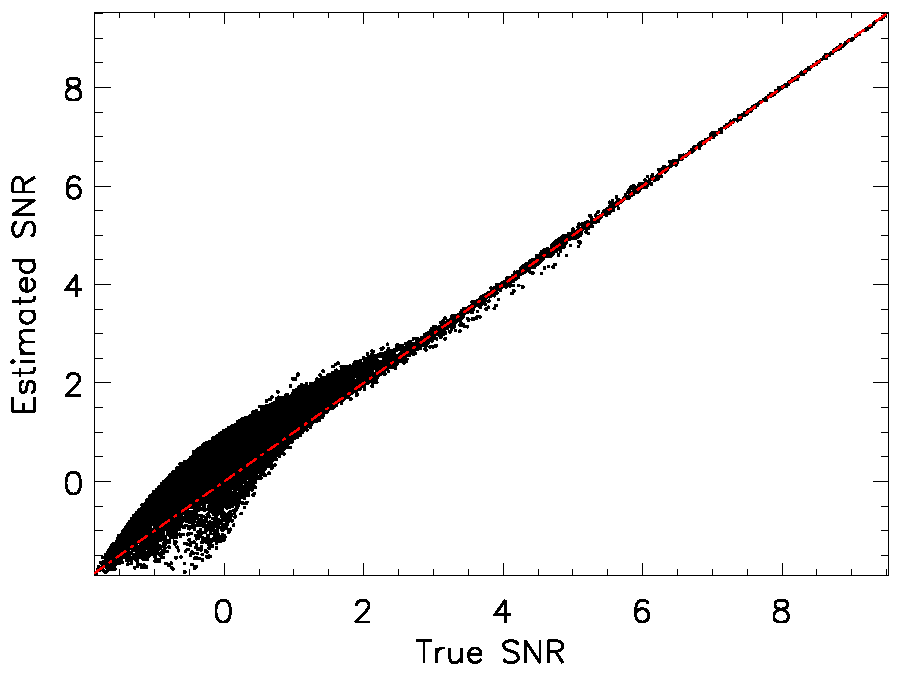
\includegraphics[width=0.45\textwidth]{Figure/Conta_noise_Grad_SNRtrueVSmeasRG377_00181_Ymap_zobs0p5_15_15_45.pdf}
\caption{\footnotesize{Comparison of the estimated GGM filtered maps signal-to-noise ratio as a function of the true signal-to-noise, using the RHAPSODY-G sub-sample. The estimated signal-to-noise is computed using the NIKA processed RHAPSODY-G sub-sample (equation \ref{eq:GGM_filter_snr}). The red dashed line represent the one to one correspondence. Each point corresponds to a pixel of the map.}}
\label{fig:noise_statistics2}
\end{figure}

%MC noise realizations
The NIKA noise is Gaussian and spatially correlated \citep{Adam2016a} but its behavior does not necessarily propagate in a trivial way under the application of the filters, especially in the case of the GGM filter, which is non-linear. In order to estimate the significance of the structures that we observe in Section~\ref{sec:Application_to_the_NIKA_clusters_sample}, we use noise realizations of the surface brightness maps generated as described in \cite{Adam2016a}. They account for the map pixel-to-pixel correlated noise induced by residual atmospheric and electronic noise, the inhomogeneities of the noise due to the scanning strategy, and the contribution of the cosmic infrared background, which is non-negligible for the deepest observations. For each cluster, we produce a set of 1000 surface brightness noise realizations, $N^{(i)}$, which are deconvolved from the transfer function associated to the NIKA data processing similarly to their corresponding cluster data and used to estimate the noise in the filtered maps using the following procedure. 

%DoG MC filter noise realizations
As the DoG filter is linear and preserves the noise Gaussianity, we process these surface-brightness-noise-only Monte Carlo realizations through the same filter as the data. Then, we estimate the respective DoG filtered maps standard deviation by taking the root-mean-square of all the processed Monte Carlo realizations, for each pixel of the map. The DoG signal-to-noise ratio are straightforwardly obtained by normalizing the filtered cluster data by the standard deviation maps, and follow Gaussian statistics.

%GGM MC filter noise realizations
According to the definition of equation \ref{eq:GGM_filter}, the noise of the GGM filtered maps depends on the surface brightness signal itself because of the non-linearity of the filter. Therefore, we use the observed signal as an estimate of the true signal, $\hat{S}$, to which we add the surface brightness noise realizations, prior to processing them through the GGM filter. The estimate of the filtered map noise contribution, from each Monte Carlo realization $i$, is then given by
\begin{equation}
	N^{(i)}_{\rm GGM} = \left(\hat{S} + N^{(i)}\right)_{\rm GGM} -  \hat{S}_{\rm GGM},
	\label{eq:GGM_filter_noise}
\end{equation}
where the index GGM corresponds to the filter application defined by equation \ref{eq:GGM_filter}. For each pixel of the map, we compute $\mu_{\rm GGM}$ and $\sigma_{\rm GGM}$, the mean and the standard deviation of the noise realizations $N^{(i)}_{\rm GGM}$ per map pixel, respectively. Accounting for the non-zero mean of the filtered map noise, the effective signal-to-noise ratio is defined as 
\begin{equation}
{\rm SNR}_{\rm GGM} = \frac{\hat{S}_{\rm GGM} - \mu_{\rm GGM}}{\sigma_{\rm GGM}}.
	\label{eq:GGM_filter_snr}
\end{equation}
In practice, the estimated surface brightness signal is the sum of the true signal, $S$, and the noise, $N$, as $\hat{S} = S + N$. In the low surface brightness signal-to-noise regions, $\hat{S}$ is therefore dominated by the noise, which can bias low the value of $\mu_{\rm GGM}$. In the case of the RHAPSODY-G sub-sample, we also dispose of the true input surface brightness signal, $\hat{S} = S$, and we use it to compute the true signal-to-noise, to quantify the reliability of our signal-to-noise estimation procedure, as discussed below.

%Figure to illustrate noise distribution
The noise distribution is illustrated in Figure \ref{fig:noise_statistics1} for both the GGM and the DoG filters. The data of \mbox{CL~J1226.9+3332} are used as an example, in the case of our baseline filter parameters (section \ref{sec:Baseline_filtering_parameters}). The histograms account for the pixels that are enclosed within 30~arcsec from the cluster center, where the noise is homogeneous. In the case of the GGM filter, we consider both the possibility in which the cluster signal, $\hat{S}$, is set to the measured signal from \mbox{CL~J1226.9+3332}, and where it is set to zero in equation \ref{eq:GGM_filter_noise}, to illustrate the noise behavior in low signal-to-noise regions. As we can see, the DoG noise statistics is described by a gaussian distribution with a mean compatible with zero, by construction. The GGM noise distribution is well described by a Gaussian distribution in signal dominated regions. However, as the signal vanishes, such as in the external regions, the noise becomes non Gaussian, its mean increases and the distribution gets positively skewed. Despite the fact that the non-zero mean of the noise is corrected for when computing the significance of the data, we note that the noise is boosted by up to 15\% (in the wing of the distribution), in the extreme case of zero signal, with respect to what one would expect for Gaussian noise.

%Figure to illustrate SNR recovery
The signal-to-noise reconstruction validation of the GGM filtered maps is illustrated in Figure~\ref{fig:noise_statistics2}, showing the estimated signal-to-noise as a function of the true signal-to-noise, computed using the RHAPSODY-G sub-sample for which both $\hat{S}$ and $S$ are available. We can observe that in the low signal-to-noise regime, the estimated signal-to-noise is overall biased high, due to the fact that $\mu_{\rm GGM}$ is biased low. At higher signal-to-noise ($\gtrsim 3$), the estimated signal-to-noise converges to the true signal-to-noise within a few percent. Our procedure is thus valid in this regime.

%Check with Rhapsody
Finally, we use the end-to-end processed and filtered maps from a RHAPSODY-G sub-sample, shown in Figure \ref{fig:RG_cluster_sample_proc}, to check that the structures we recover are reliable. Indeed, above 3, the signal-to-noise of the recovered features is consistent with what we expect in the case of the raw maps of Figure \ref{fig:RG_cluster_sample} when using the true signal-to-noise.

%==================== Point sources
\subsection{Point sources residuals}
\begin{figure}[h]
\centering
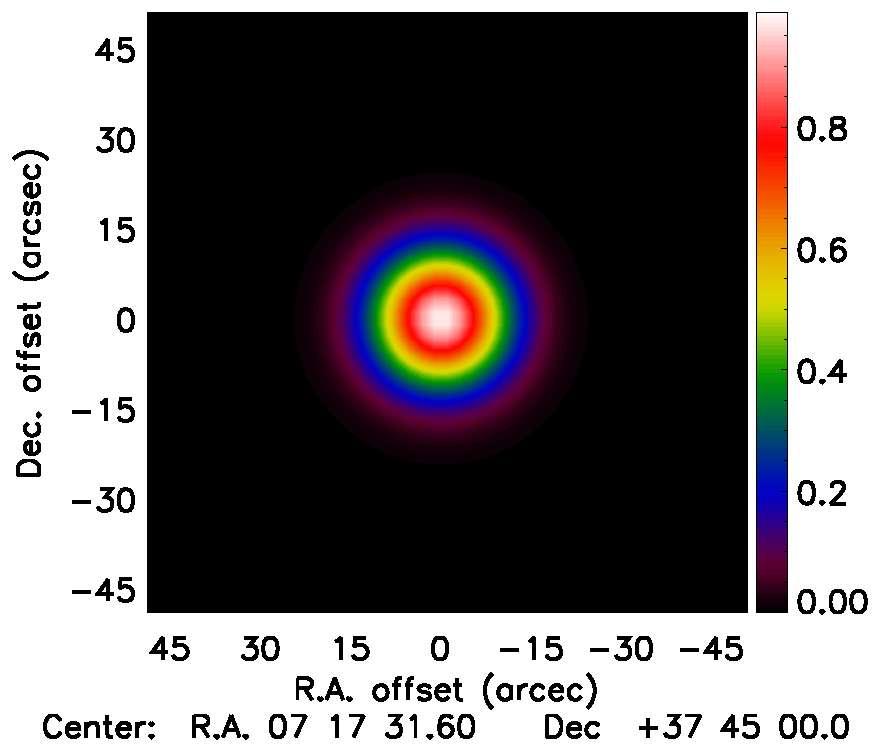
\includegraphics[trim=0cm 0.7cm 0cm 0cm, clip=true, totalheight=3.4cm]{Figure/PSalone_Input_PointSource_15_15_45.pdf}
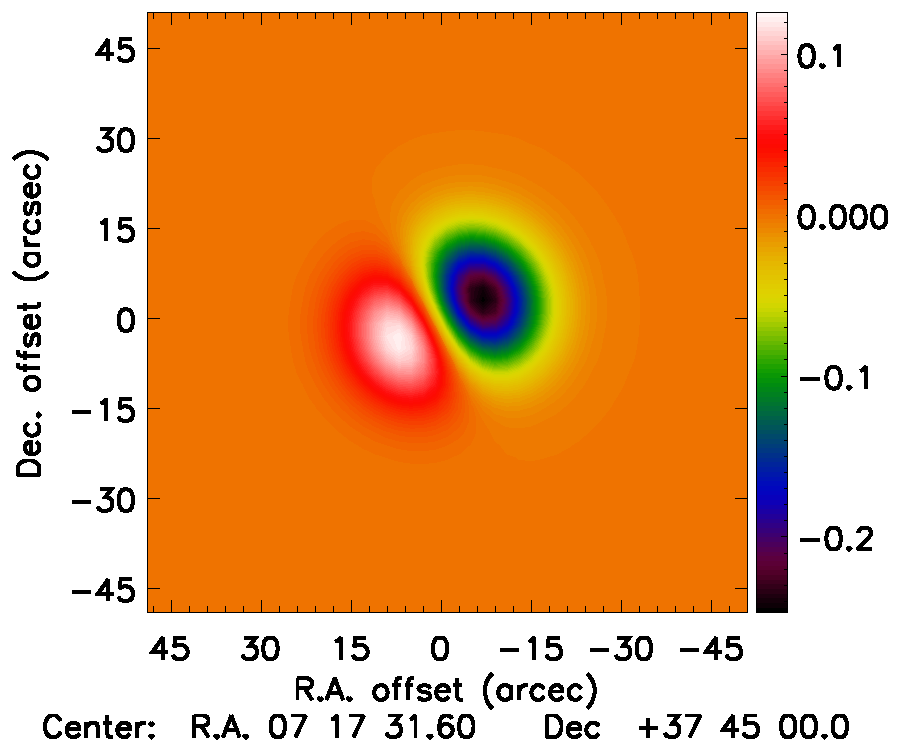
\includegraphics[trim=0cm 0.7cm 0cm 0cm, clip=true, totalheight=3.4cm]{Figure/PSalone_Input_PointSourceResidual_15_15_45.pdf}
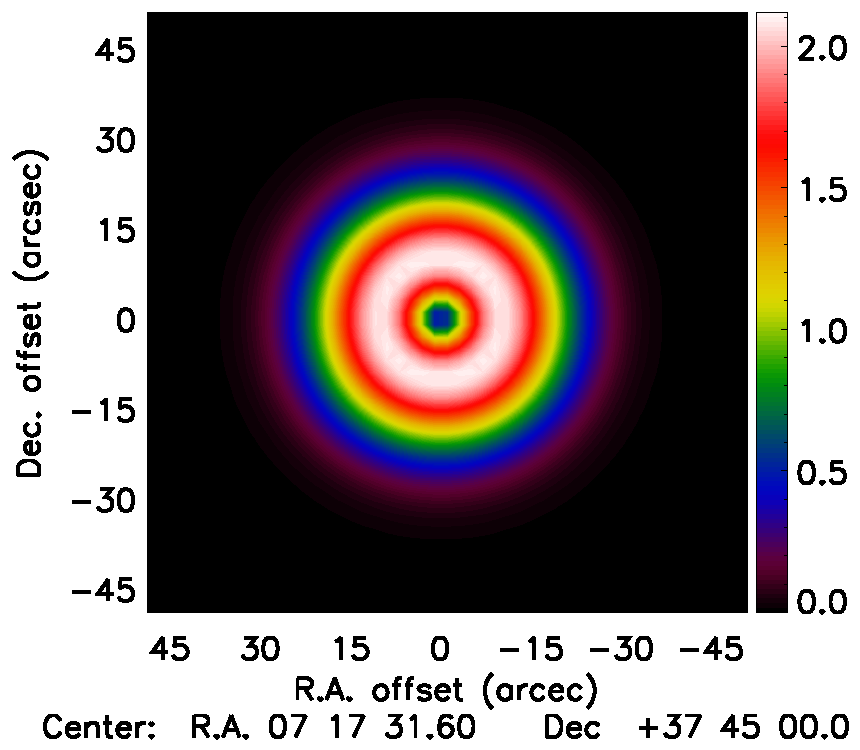
\includegraphics[trim=0cm 0.7cm 0cm 0cm, clip=true, totalheight=3.4cm]{Figure/PSalone_GGM_PointSource_15_15_45.pdf}
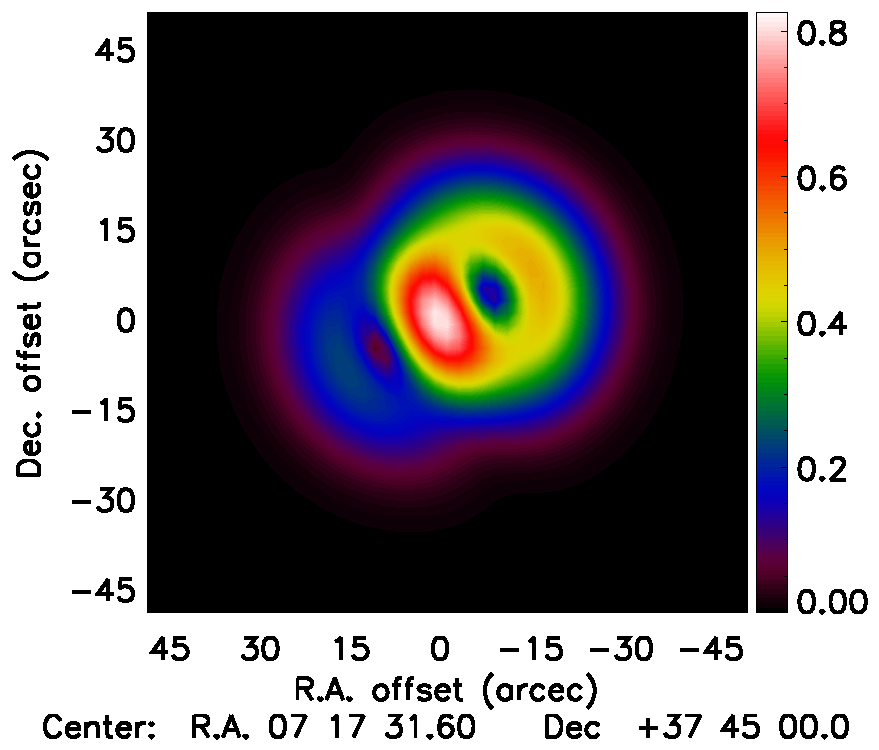
\includegraphics[trim=0cm 0.7cm 0cm 0cm, clip=true, totalheight=3.4cm]{Figure/PSalone_GGM_PointSourceResidual_15_15_45.pdf}
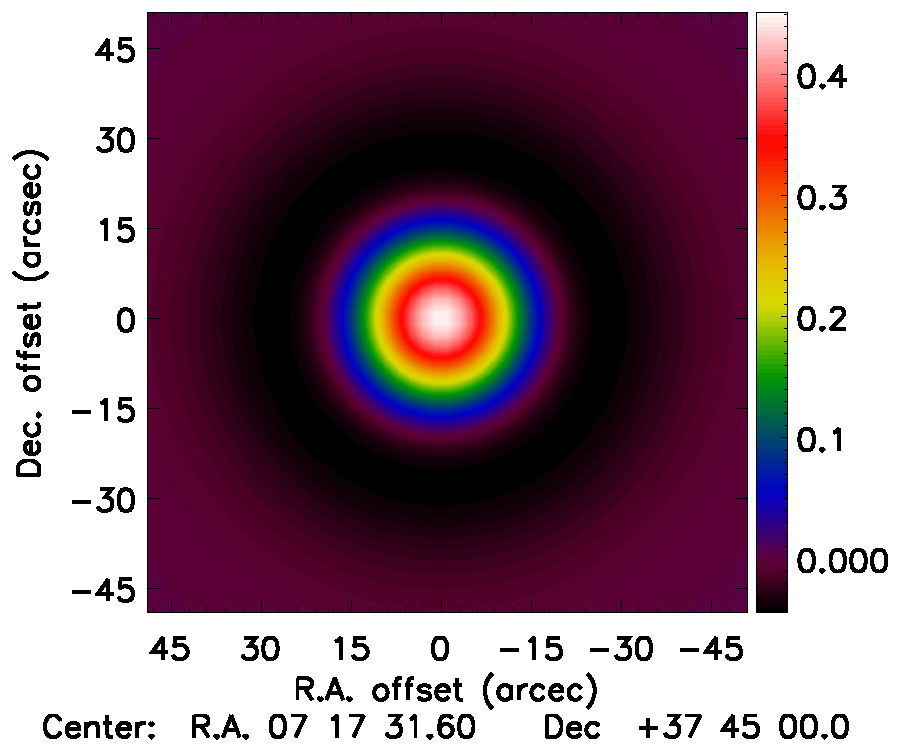
\includegraphics[trim=0cm 0.7cm 0cm 0cm, clip=true, totalheight=3.4cm]{Figure/PSalone_DoG_PointSource_15_15_45.pdf}
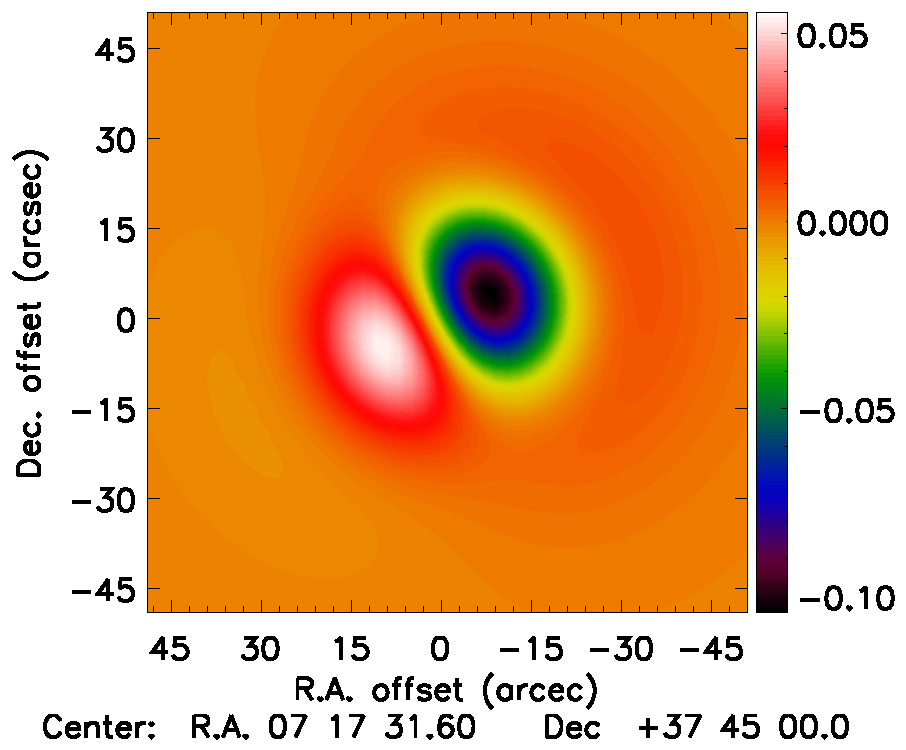
\includegraphics[trim=0cm 0.7cm 0cm 0cm, clip=true, totalheight=3.4cm]{Figure/PSalone_DoG_PointSourceResidual_15_15_45.pdf}
\caption{\footnotesize{Application of the filters to point source residuals in case 1 (no source subtraction, left) and case 2 (source improperly subtracted, right). The input point source flux has been normalized to one. {\bf Top}: input surface brightness map. {\bf Middle}: GGM filtered map. {\bf Bottom}: DoG filtered map.}}
\label{fig:Point_source_maps}
\end{figure}
Foreground, background, or cluster-member galaxies can show up as point sources in tSZ images, which constitutes a well know potential bias. In the case of NIKA, these sources are subtracted either by fitting their flux together with the tSZ signal \citep{Adam2015}, or by modeling their Spectral Energy Distribution (SED) and fitting them to multi-wavelength photometric data to extrapolate their flux in the respective NIKA bands \citep[see the method detailed in][]{Adam2016a}. Even if such procedures provides a first good estimate of the contaminant, they are limited by the accuracy of the model to describe the data, the limited available extra data, and miscentering arising from limited accuracy in the source coordinate or telescope pointing precision. At 150 GHz, the contaminant sources are mostly radio galaxies, but infrared galaxies can also have a significant contribution.

We estimate the impact of residual point sources by considering the following approach in two upper limit cases:
\begin{enumerate} 
\item Point sources below the detection threshold that are not subtracted. We simulate point sources with a flux of $3 \sigma$ that of the noise rms, and assume that it is not subtracted from the tSZ map. 
\item Point sources that are poorly subtracted. We simulate a 3 mJy point source (the typical flux of the brightest radio sources observed in the NIKA clusters at 150 GHz), which we subtract assuming a flux that is off by 10\%, and including a miscentering offset of 3 arcsec \citep[the NIKA pointing accuracy for one scan][]{Catalano2014}.
\end{enumerate}
As the GGM filter is not linear, the point source contamination induced by the application of the filter depends not only on the point sources themselves, but also on the local environment of the source. Therefore, we test both the case where the sources are simulated in the outskirts of the clusters, where the noise dominates, and within a few arcsec of the cluster core, where the signal dominates.

Using our baseline filter parameters, we find that the difference between the point source contaminated and the tSZ only maps can reach deviations of up to $4 \sigma$, both for the GGM and the DoG filters. As the signal-to-noise ratio of the simulated clusters is set to match the highest signal-to-noise NIKA cluster, it represents an upper limit of the contamination. In addition, the biases remain local on the maps and exhibit specific structures that are distinct from the ones that appear in the case of interacting clusters (ring-like shaped, azimuthally symmetric, or dipole-like at the scale of the filter, see figure \ref{fig:RG_cluster_sample}). Nonetheless, point source residuals could mimic compact tSZ cores, at the scale of the beam. As we increase the filter scales, the signal arising from point source residuals quickly becomes insignificant. The signatures of point source residuals are illustrated in figure \ref{fig:Point_source_maps}. Due to the GGM non linearity, the corresponding extra signal arising from point sources can slightly deviate from the one shown in figure \ref{fig:Point_source_maps}.

We conclude that undetected or mismodeled point sources are an unavoidable potential bias. They can affect the interpretation of the signal at a level of a few $\sigma$, but they cannot lead to a mis-interpretation of the overall signal observed in tSZ maps as the contamination remains local.

%###############################################################################################
%##########################                             Application to NIKA                           ##########################
%###############################################################################################
\section{Application to the NIKA clusters sample}\label{sec:Application_to_the_NIKA_clusters_sample}
%==================== Data
\subsection{NIKA data}\label{sec:NIKA_Data}
NIKA has been used to map six clusters of galaxies using the tSZ effect at 150 and 260 GHz between November 2012 and February 2015. This sample contains both well known objects various with multi-wavelength coverage and Planck discovered sources, at intermediate and high redshifts. It was designed to provide pilot observations to test the feasibility of the NIKA2 tSZ Large Program, which is under preparation \citep{Comis2016}. The main steps of the data reduction are described in \cite{Adam2014,Adam2015}. In this paper, we use the NIKA 150 GHz tSZ maps only, deconvolved from the transfer function except for the beam smoothing (see section \ref{sec:Transfer_function_filtering}). The overall calibration uncertainty is estimated to be about 10\% depending on the observation campaign (see table \ref{tab:cluster_summary}), including the brightness temperature model of our primary calibrator, the NIKA bandpass uncertainties, the opacity correction, and the stability of the instrument \citep{Catalano2014}. All the clusters are contaminated by foreground and/or background galaxies that appear as point sources in the maps and they are removed according to the procedure described in \cite{Adam2015} and \cite{Adam2016a}. 

The NIKA surface brightness maps at 150 GHz are provided in Figure \ref{fig:NIKA_cluster_sample} and the main properties of the clusters are listed in Table \ref{tab:cluster_summary}. We can observe a wide variety of cluster morphologies, spanning redshifts between 0.45 and 0.89. The peak signal-to-noise, at a 22 arcsec FWHM resolution, depends strongly on the observing time and weather conditions, ranging from $\sim 4 \sigma$ to about $20 \sigma$ for the deepest observations. The RHAPSODY-G processed tSZ maps of Figure \ref{fig:RG_cluster_sample_proc} present signal-to-noise ratio comparable to that of the deepest NIKA data of \mbox{MACS~J0717.5+3745} and \mbox{CL~J1226.9+3332}. We thus expect to be able to find sub-structure features at a similar significance within these two clusters. Details specific to individual clusters are given in the following sub-sections.

\begin{table*}[]
\caption{\footnotesize{Summary of the main properties of the NIKA cluster sample, ordered by increasing redshift.}}
\begin{center}
\resizebox{\textwidth}{!} {
\begin{tabular}{c|c|c|c|c|c||c|c|c|c}
\hline
\hline
Name & $z$ & kpc/arcsec & $M_{500}$ & $Y_{500}$ & Comments & Configuration & Calibration uncertainty & Projected time & Central rms$^{(b)}$ \\
 &  & & ($10^{14}$ M$_{\odot}$)& ($10^{-3}$arcmin$^2$) & & & & (hour) & (mJy/beam) \\
\hline
RX~J1347.5-1145 & 0.452 & 5.9 & 11.0 & 1.40 & Cool-core+merger & Nov. 2012, preliminary instrument & 15\% & 5.8 & 1.2 \\ 
MACS~J1423.8+2404 & 0.545 & 6.6 & 4.9 $^{(a)}$ & 0.47 $^{(a)}$ & Relaxed elliptical cool-core & Feb. 2014, Open Pool & 7\% &1.5 & 0.35 \\ 
MACS~J0717.5+3745 & 0.546 & 6.6 & 11.5 & 1.74 & Multiple merger, strong kSZ & Jan./Feb. 2014 \& 2015, Open Pool & 7\% & 13.1 & 0.10 \\ 
PSZ1~G046.13+30.75 & 0.569 & 6.7 & 6.4 & 0.70 & Disturbed & Nov. 2015, Open Pool & 9\% & 6.0 &  0.32\\ 
PSZ1~G045.85+57.71 & 0.611 & 6.9 & 7.0 & 0.92 & Elliptical cool-core & Nov. 2015, Open Pool & 9\% & 6.4 & 0.17 \\ 
CL~J1226.9+3332 &  0.888 & 8.0 & 5.7 & 0.90 & Disturbed core & Feb. 2014, Open Pool & 7\% & 7.8 & 0.17 \\ 
\hline
\end{tabular}
}
\end{center}
{\small {\bf Notes.} The masses are extracted from the {\textit Planck} catalog \citep{PlanckXXVII2015}. The integrated Compton parameter, $Y_{500}$, is computed by normalizing $Y_{5R_{500}}$ (extracted from the {\textit Planck} catalog) by a factor of 1.79, assuming a Universal pressure profile \citep{Arnaud2010}. $^{(a)}$ From \cite{Adam2016a}, as this cluster is not in the {\textit Planck} catalog. $^{(b)}$ At the 22 arcsec FWHM effective angular resolution.}
\label{tab:cluster_summary}
\end{table*}

\begin{figure*}[h]
\resizebox{\textwidth}{!} {
\begin{tabular}{cccccc}
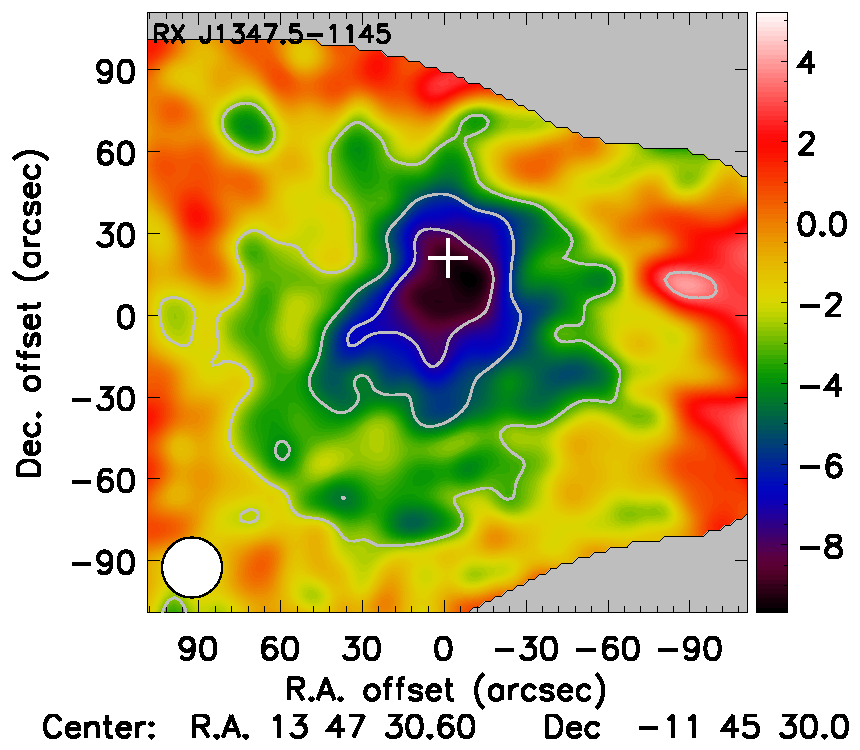
\includegraphics[trim=0cm 0cm 0cm 0cm, clip=true, totalheight=5.9cm]{Figure/Map_RXJ1347.pdf} & 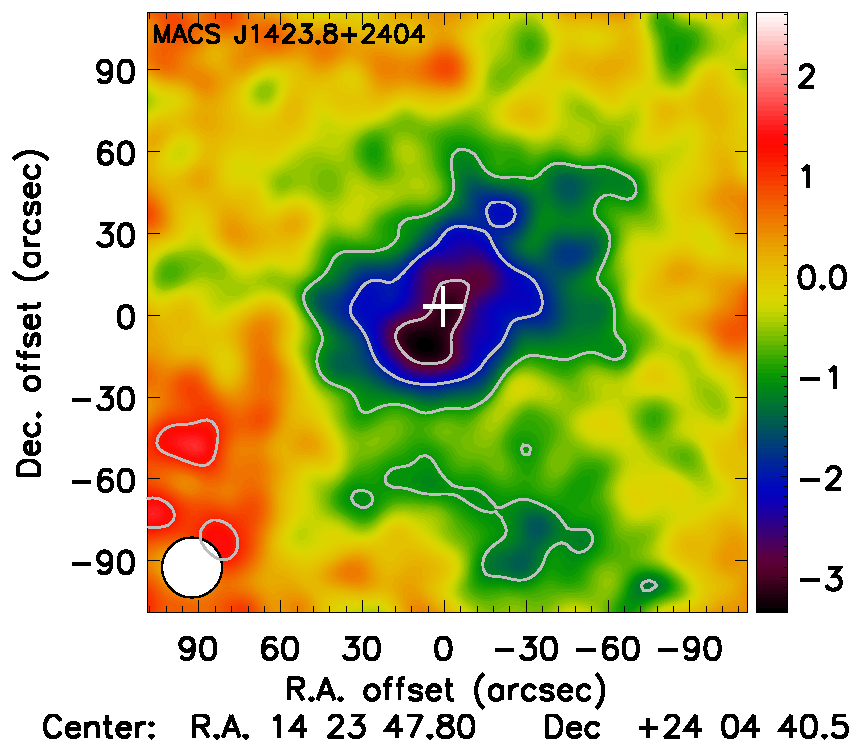
\includegraphics[trim=2.45cm 0cm 0cm 0cm, clip=true, totalheight=5.9cm]{Figure/Map_MACSJ1424.pdf} & 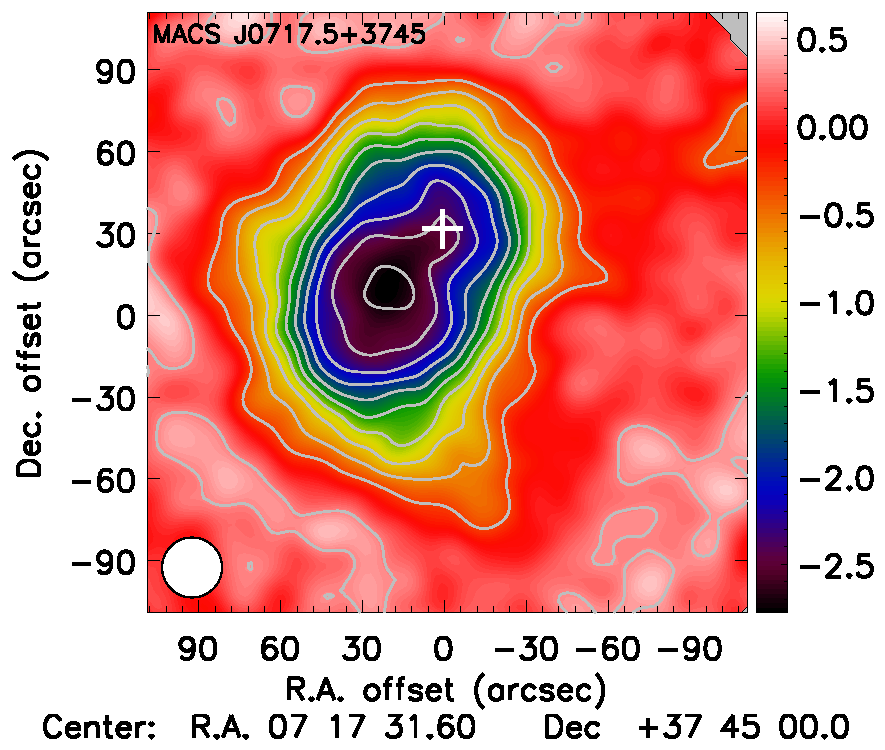
\includegraphics[trim=2.45cm 0cm 0cm 0cm, clip=true, totalheight=5.9cm]{Figure/Map_MACSJ0717.pdf} & 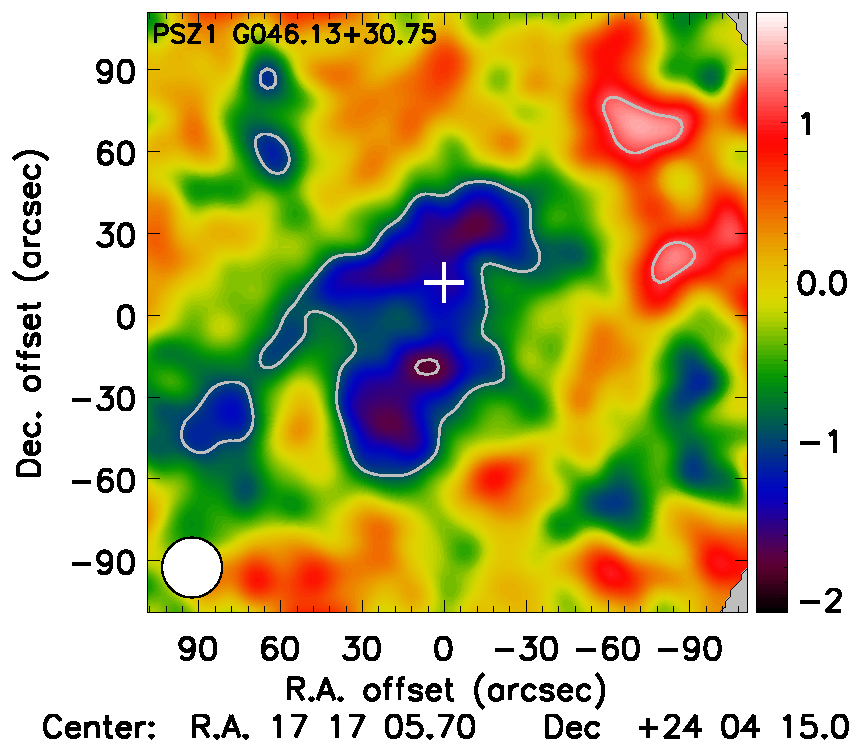
\includegraphics[trim=0cm 0cm 0cm 0cm, clip=true, totalheight=5.9cm]{Figure/Map_PSZ1G046.pdf} & 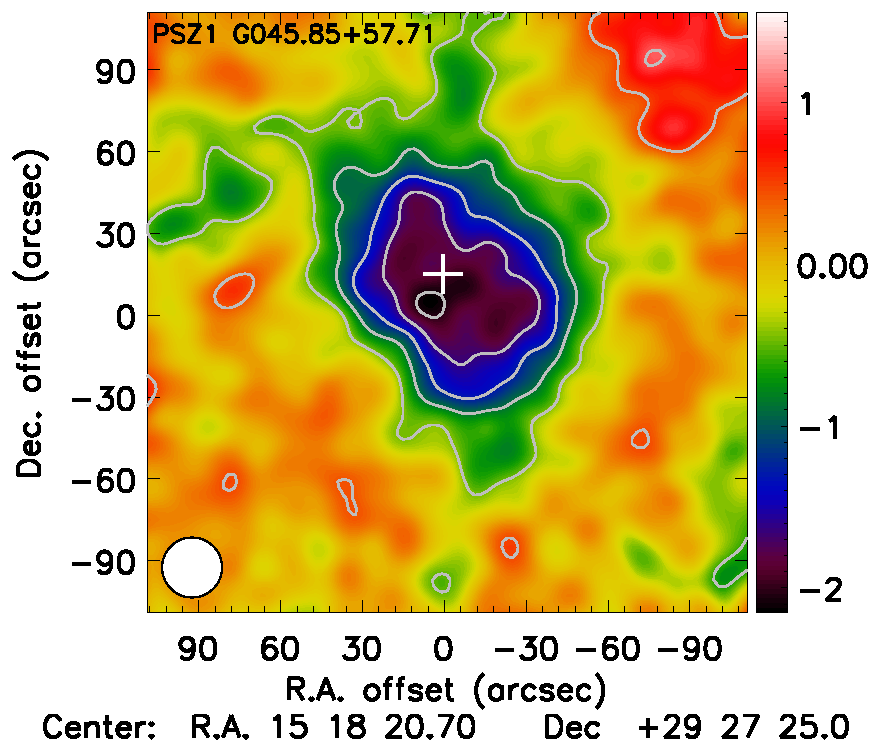
\includegraphics[trim=2.45cm 0cm 0cm 0cm, clip=true, totalheight=5.9cm]{Figure/Map_PSZ1G045.pdf} & 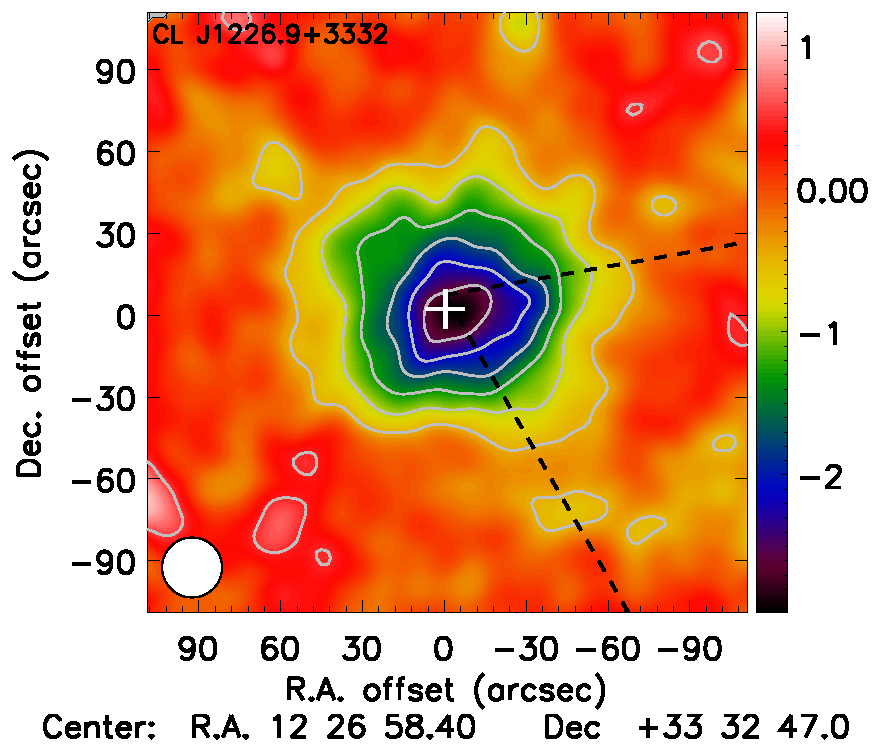
\includegraphics[trim=2.45cm 0cm 0cm 0cm, clip=true, totalheight=5.9cm]{Figure/Map_CLJ1227.pdf} \\
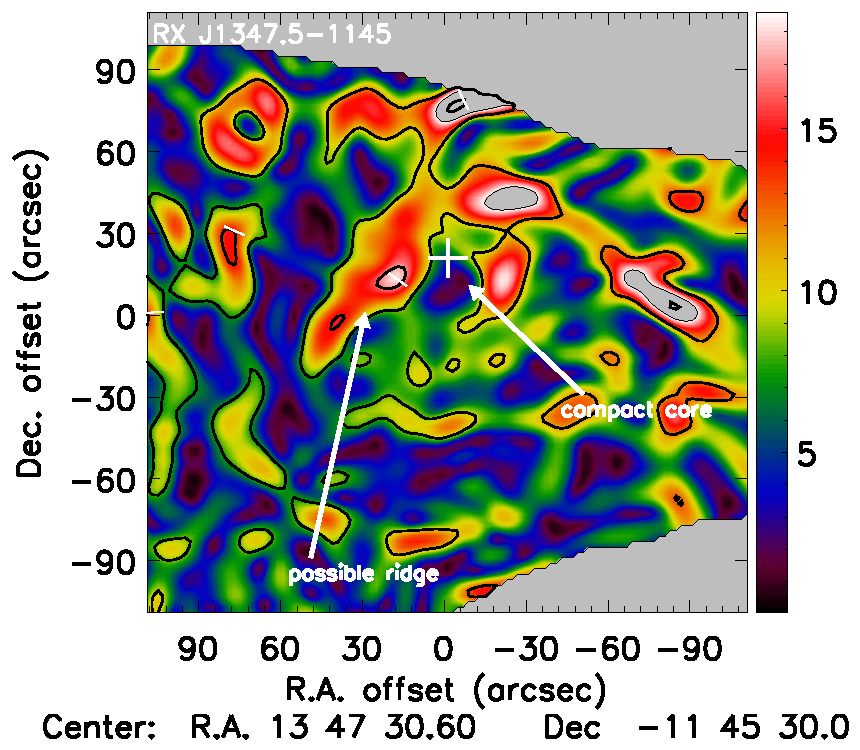
\includegraphics[trim=0cm 0cm 0cm 0cm, clip=true, totalheight=5.9cm]{Figure/Grad_RXJ1347_15_15_45.pdf} & 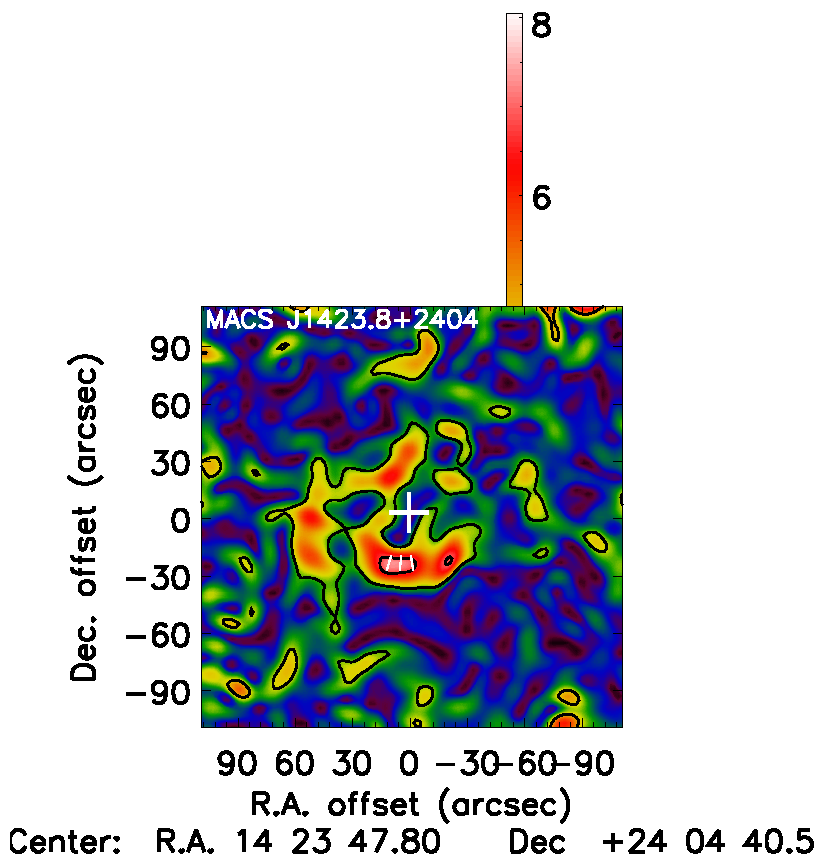
\includegraphics[trim=2.45cm 0cm 0cm 0cm, clip=true, totalheight=5.9cm]{Figure/Grad_MACSJ1424_15_15_45.pdf} & 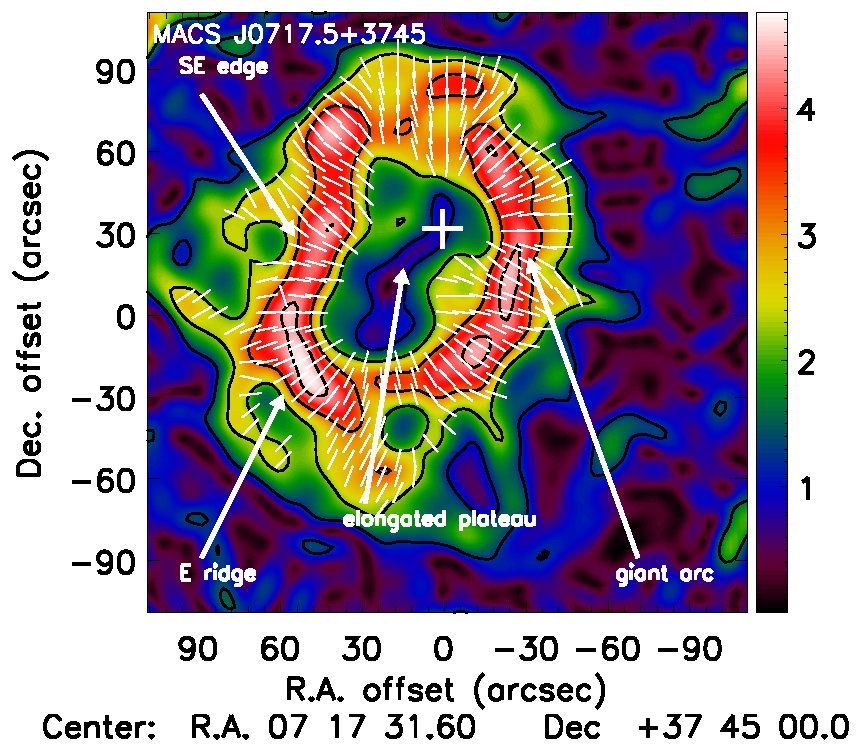
\includegraphics[trim=2.45cm 0cm 0cm 0cm, clip=true, totalheight=5.9cm]{Figure/Grad_MACSJ0717_15_15_45.pdf} & 
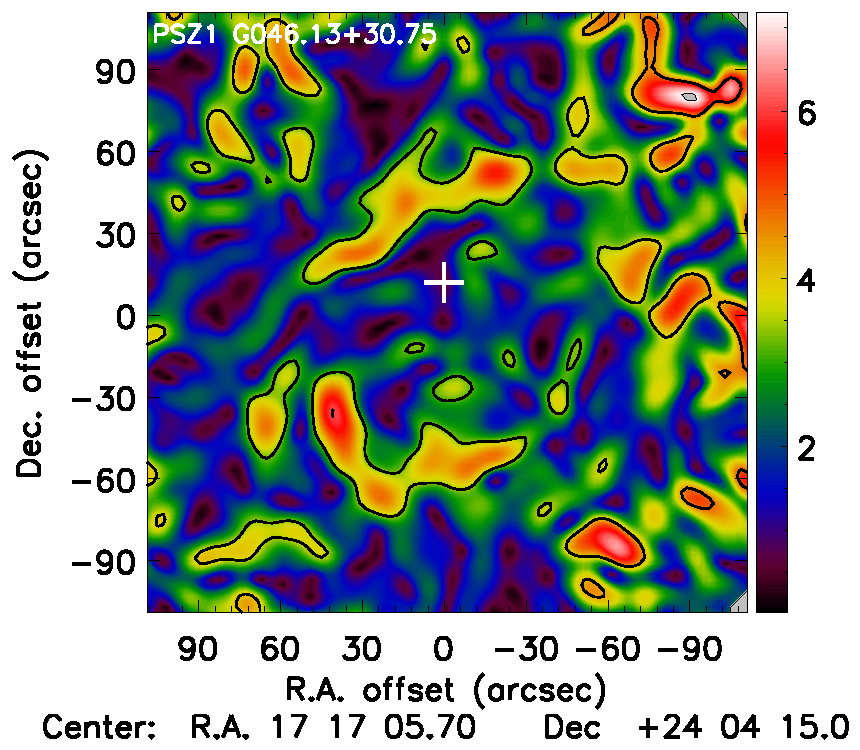
\includegraphics[trim=0cm 0cm 0cm 0cm, clip=true, totalheight=5.9cm]{Figure/Grad_PSZ1G046_15_15_45.pdf} & 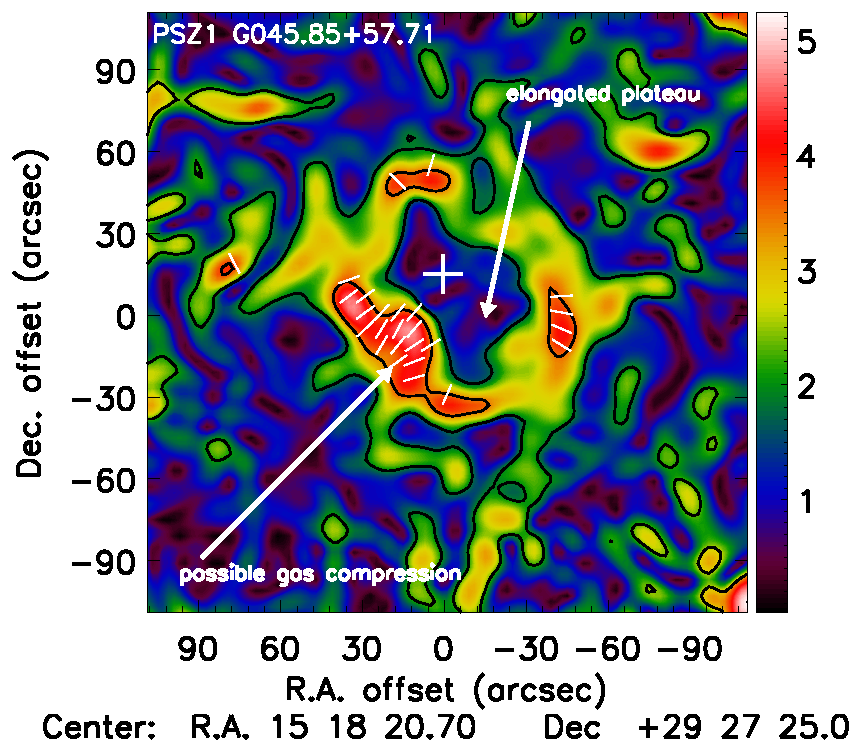
\includegraphics[trim=2.45cm 0cm 0cm 0cm, clip=true, totalheight=5.9cm]{Figure/Grad_PSZ1G045_15_15_45.pdf} & \includegraphics[trim=2.45cm 0cm 0cm 0cm, clip=true, totalheight=5.9cm]{Figure/Grad_CLJ1227_15_15_45.pdf} \\
\includegraphics[trim=0cm 0cm 0cm 0cm, clip=true, totalheight=5.9cm]{Figure/DoG_RXJ1347_15_15_45.pdf} & \includegraphics[trim=2.45cm 0cm 0cm 0cm, clip=true, totalheight=5.9cm]{Figure/DoG_MACSJ1424_15_15_45.pdf} & \includegraphics[trim=2.45cm 0cm 0cm 0cm, clip=true, totalheight=5.9cm]{Figure/DoG_MACSJ0717_15_15_45.pdf} & 
\includegraphics[trim=0cm 0cm 0cm 0cm, clip=true, totalheight=5.9cm]{Figure/DoG_PSZ1G046_15_15_45.pdf} & \includegraphics[trim=2.45cm 0cm 0cm 0cm, clip=true, totalheight=5.9cm]{Figure/DoG_PSZ1G045_15_15_45.pdf} & \includegraphics[trim=2.45cm 0cm 0cm 0cm, clip=true, totalheight=5.9cm]{Figure/DoG_CLJ1227_15_15_45.pdf}\\
\end{tabular}
}
\caption{\footnotesize{Redshift-ordered maps of the NIKA cluster sample at 150 GHz. 
{\bf Top:} Surface brightness images. Each map has been smoothed to an effective angular resolution of 22 arcsec FWHM, as shown by the bottom left white circle. Point sources have been subtracted and the data have been deconvolved from the transfer function, but the zero level absolute brightness remains unconstrained. 
{\bf Middle:} GGM filtered maps.
{\bf Bottom:} DoG filtered maps.
In all cases, contours provide the signal-to-noise ratio, starting at $\pm 2 \sigma$ and increasing by $2 \sigma$ steps. The white crosses provide the main X-ray peak (see Table \ref{tab:xray_peak}). In the case of \mbox{MACS~J0717.5+3745}, the kSZ contribution is not accounted for in the map presented here (see section \ref{sec:MACSJ0717} for more details).
}}
\label{fig:NIKA_cluster_sample}
\end{figure*}

\begin{table}[]
\caption{\footnotesize{Coordinates of the main X-ray peak.}}
\begin{center}
\resizebox{0.5\textwidth}{!} {
\begin{tabular}{c|c|c|c}
\hline
\hline
Name & R.A. & Dec. & Reference \\
\hline
RX~J1347.5-1145 & 13:47:30.575 & -11:45:10.08 & {\textit Chandra} (ObsID3592) \\ 
MACS~J1423.8+2404 & 14:23:47.908 & +24:04:42.69 & {\textit Chandra} (ObsID4195) \\ 
MACS~J0717.5+3745 & 07:17:31.740 & +37:45:30.73 & {\textit Chandra} (ObsID4200) \\ 
PSZ1~G046.13+30.75 & 17:17:05.780 & +24:04:26.00 & {\textit XMM-Newton} (ObsID0693661401) \\ 
PSZ1~G045.85+57.71 & 15:18:20.811 & +29:27:39.10 & {\textit XMM-Newton} (ObsID0693661101) \\ 
CL~J1226.9+3332 & 12:26:58.454 & +33:32:48.36 & {\textit Chandra} (ObsID5014) \\ 
\hline
\end{tabular}
}
\end{center}
\label{tab:xray_peak}
\end{table}

%==================== Low significance
\subsection{Low significance sub-sample}
The three clusters \mbox{RX~J1347.5-1145}, \mbox{MACS~J1423.8+2404} and \mbox{PSZ1~G046.13+30.75} have been imaged with NIKA. Despite the relatively low significance of this sub-sample (less than 10 $\sigma$ per beam at the 22 arcsec resolution), we apply the GGM and DoG filter to the maps. We observe hints for internal structures, but only at low significance level, as briefly discussed below.

% RXJ1347
\subsubsection{RX~J1347.5-1145}\label{sec:RXJ1347.5-1145}
\mbox{RX~J1347.5-1145} is a massive cluster at redshift 0.45, and one of the most luminous X-ray cluster. Being an extremely bright tSZ source, it has already been observed using the tSZ effect by several groups \citep[e.g.][]{Pointecouteau1999,Komatsu1999,Mason2010,Plagge2012,Adam2014,Sayers2016,Kitayama2016}. \mbox{RX~J1347.5-1145} presents a dense core, but also shows an extension toward the southeast, that is associated with the merger of a subcluster. The tSZ peak is aligned with the southeast extension, corresponding to the overpressure caused by the shock in this region. This cluster was observed with an early setup of the NIKA instrument \citep[bandpass, sensitivity, calibration procedure, see][for more details]{Adam2014}. In addition, the scanning strategy was not isotropic due to a mistake in the control software, leading to possible artifacts in the filtered map. Therefore, the application of the filtering algorithms on the NIKA map of \mbox{RX~J1347.5-1145} is meant to remain qualitative in this paper (see section \ref{sec:Filtered_maps_of_RXJ1347.5-1145} for the maps). The GGM filtered map presents a $\gtrsim 2 \sigma$ ridge ($\gtrsim 4 \sigma$ when using $\theta_0 = 20$ arcsec), inclined by 40 degrees with respect to the Dec. axis, about 30 arcsec (178 kpc) east from the X-ray center. It could be associated to the sub-structures seen in {\textit Chandra} data by \cite{Kreisch2016}, but deeper tSZ observation are necessary to confirm it. The DoG filtered map shows that the tSZ pressure in the cluster core is elongated from SE to NW. Large scales being filtered out, the morphology of the map compares well with that of MUSTANG \citep{Mason2010} and ALMA \citep{Kitayama2016} that are sensitive to smaller scales and intrinsically filter out large scales.

%MACSJ1424
\subsubsection{MACS~J1423.8+2404}
\mbox{MACS~J1423.8+2404} is a very relaxed system and a typical cool-core, at redshift 0.55. The corresponding NIKA observations and data reduction are detailed in \citep{Adam2016a}, including a detailed description of the cluster. The peak signal-to-noise ratio of the NIKA map reaches about 6 at the 22 arcsec resolution. The GGM and DoG maps do not allow us to identify sub-structures that deviate from that expected for a spherically symmetric object, within the noise fluctuations that are large.

% PSZ1G046
\subsubsection{PSZ1~G046.13+30.75}
\mbox{PSZ1~G046.13+30.75} is a {\textit Planck} discovered cluster \citep{PlanckXXIX2014}, at redshift 0.55, and was observed during the same campaign as another NIKA cluster, \mbox{PSZ1~G045.85+57.71} \citep[see][for more details]{Ruppin2016}. The observing weather conditions were unstable with a high opacity and the cluster significance barely reaches $4 \sigma$ per 22 arcsec FWHM beam at the peak on the NIKA map. The GGM and DoG filtered maps are consistent with noise.

%==================== High significance
\subsection{High significance sub-sample}
The three other NIKA clusters, \mbox{MACS~J0717.5+3745}, \mbox{PSZ1~G045.85+57.71} and \mbox{CL~J1226.9+3332}, present a peak significance larger than 10 $\sigma$ at the 22 arcsec resolution, with a maximum of more than $18 \sigma$ for \mbox{MACS~J0717.5+3745} (see figure \ref{fig:NIKA_cluster_sample}). They allow us to investigate in more depth the inner structure of the clusters. The GGM and DoG filtered maps of these data are presented in Figure \ref{fig:filtered_NIKA_maps} for our baseline filter parameters.

%---------- MACSJ0717
\subsubsection{MACS~J0717.5+3745}\label{sec:MACSJ0717}
\mbox{MACS~J0717.5+3745} is one of the most disturbed clusters known to date. It is made of at least four interacting sub-clusters \citep{Ma2009}, and is thus an excellent target to search for discontinuities and secondary peaks in tSZ maps. In addition to the systematic uncertainties discussed in section \ref{sec:Systematics_and_noise_properties}, \mbox{MACS~J0717.5+3745} contains a significant amount of kinetic Sunyaev-Zel'dovich \citep[kSZ,][]{Sunyaev1980} signal and it is the only cluster for which an individual kSZ detection has been obtained to date \citep[][]{Mroczkowski2012,Sayers2013,Adam2016b}. The kSZ signal is related to the gas density and line-of-sight velocity and has to be subtracted in order to study the pressure structure via the tSZ signal. \cite{Mroczkowski2012}, \cite{Sayers2013} and \cite{Adam2016b} have obtained several kSZ signal models, but they are all limited by the large uncertainties in their best-fit parameters and are subject to strong assumptions in the gas modelling. Therefore, it is only possible to test the impact of the kSZ signal on our result by comparing the recovered sub-structures in the cases with and without kSZ correction. We thus produce a kSZ clean map of \mbox{MACS~J0717.5+3745} using the best-fit kSZ model from \cite{Adam2016b} to do so.

The disturbed dynamical state of \mbox{MACS~J0717.5+3745} is obvious, as can be observed in Figure \ref{fig:NIKA_cluster_sample}, and is discussed in details in \cite{Adam2016b}, where the impact of the kSZ signal on the 150 GHz image is also addressed. The overall structure of the GGM and the DoG maps are the same for the case with and without kSZ, but the relative amplitude of the structures strongly depends on the correction. Therefore, the kSZ contaminant only allows us for a qualitative estimate of the gas inner structure. The GGM maps present two strong ridges on the east and southeast regions, of $\sim 1$ arcmin (395 kpc) each (${\rm SNR}_{\rm GGM} > 8$). In addition, we observe a large arc ($\sim 90$ arcsec) in the west sector. We note that the eastern ridge is nearly aligned with a radio relic \citep[see, e.g.][]{vanWeeren2017}, and both could be sourced by a shock caused by the ongoing merger. The null of the gradient extends across all the brightest regions of the cluster in the case without kSZ correction, while it presents two nulls for the kSZ cleaned version of the map. In both cases, the main X-ray peak is aligned with a null region of the gradient, but we note that the the X-ray structure is itself complex and presents several peaks \citep[e.g.][]{Ma2009}. Both DoG maps highlight the presence of two main peaks in the pressure distribution (at $> 4 \sigma$). This was also observed by \cite{Mroczkowski2012} using MUSTANG data. One of the peaks nearly coincides with the main X-ray peak while the other one is coincident with the most massive sub-cluster, as identified from a strong lensing reconstruction \citep[e.g.][]{Limousin2015}. It is also the location of the hottest region that shows adiabatically compressed gas from the merger of the two main clusters \citep[see][]{Adam2016b}.

The GGM and DoG filtered maps of \mbox{MACS~J0717.5+3745} compare well to multiple major mergers as identified in the RHAPSODY-G simulation. They provide further insight into the gas structure of the cluster, with respect to the surface brightness image, by allowing us to identify regions of compressed gas. They are consistent with a major merger of two main sub-clusters and that of one (or more) additional sub-cluster likely to be smaller. Nevertheless, projection effects limit our interpretation of the data, in particular in the case of such a complex object. Using the filtered maps together with multi-wavelength data might in the future provide a better understanding of the ongoing merger scenario.

%---------- PSZ1G045
\subsubsection{PSZ1~G045.85+57.71}
\mbox{PSZ1~G045.85+57.71} is a {\textit Planck} discovered cluster \citep{PlanckXXIX2014}, at redshift 0.61, and was observed during the same campaign as \mbox{PSZ1~G046.13+30.75} \citep[see][for more details]{Ruppin2016}. It was classified as a cool-core cluster based on its temperature and entropy profile, both fully consistent with the \rexcess\ cool-core sub-sample \citep{Bohringer2007,Arnaud2010,Pratt2010}. Its morphology is highly elliptical, with a main axis oriented about 45 degrees with respect to the R.A. axis, as can be observed in Figure \ref{fig:NIKA_cluster_sample}, but \cite{Ruppin2016} do not find evidence for merging activity. The tSZ peak is consistent with that of the X-ray, and the tSZ elongation is mostly prominent toward the southwest.

The GGM map of \mbox{PSZ1~G045.85+57.71} is that of an elongated ring following the morphology of the cluster. On the southeast region, we observe a stronger pressure gradient extending over about 45 arcsec (312 kpc) and reaching ${\rm SNR}_{\rm GGM} = 5.8$. In contrast to the RHAPSODY-G relaxed cluster RG361\_00188, the GGM map shows that the pressure is approximately constant along the line-of-sight, over a wide area from the X-ray core to the southwest extension. As \mbox{PSZ1~G045.85+57.71} is a cool-core cluster, with a dense X-ray core, this indicates that the temperature rises in the southwest sector. The DoG map does not show the presence of any strong core and is consistent with the pressure being relatively constant from the X-ray core to the southwest extension. As a consequence of the lack of signal on small scales, the DoG map significance is relatively low, reaching only $4 \sigma$ at the peak. The main peak is located within a few arcsec of the X-ray core, but two secondary peaks are visible towards the southwest and on the north.

The GGM and DoG images of \mbox{PSZ1~G045.85+57.71} are consistent with that of a merging sub-group falling from the southwest to the main cluster. It would be responsible for the local temperature rise and the gas compression on the southwest. Such scenarios are commonly observed in the RHAPSODY-G clusters. In contrast, relaxed RHAPSODY-G systems do not present similar features in their filtered maps, which reinforces the interpretation proposed above. Nevertheless, we note that the signal-to-noise ratio remains limited in the case of this cluster, and any stronger conclusions would require deeper data.

%---------- CLJ1227
\subsubsection{CL~J1226.9+3332}
\mbox{CL~J1226.9+3332} is a hot and massive high redshift cluster, at $z=0.89$. It was discovered by ROSAT \citep{Ebeling2001} and has been the object of several multi-wavelength studies since then. In particular, \cite{Maughan2007} identified a temperature excess in the southwest region from {\textit XMM-Newton} and {\textit Chandra} X-ray observations, in agreement with a tSZ ridge observed by MUSTANG \citep{Korngut2011}. This extension seen in the gas distribution is attributed to the merging of a smaller cluster that is visible from Hubble lensing data \citep{Jee2009}. NIKA was used to map the tSZ signal toward \mbox{CL~J1226.9+3332} as discussed in \cite{Adam2015}, who also found an extension in the southwest region when subtracting a spherical model fitted to their data.

The large scale morphology of the NIKA map presented in Figure \ref{fig:NIKA_cluster_sample} shows that \mbox{CL~J1226.9+3332} is overall spherical and we observe a good match between the X-ray and tSZ peaks. This is confirmed by the GGM filtered map (Figure \ref{fig:filtered_NIKA_maps}), where the location of the null of the gradient, at the tSZ peak, is in excellent agreement with the X-ray peaks. The gradient is strong around the core, indicating the presence of a compact pressure structure. However, we observe a strong gradient ridge in the southwest region (${\rm SNR}_{\rm GGM} = 5.7$), extending over about 45 arcsec (360 kpc). The DoG map agrees with \mbox{CL~J1226.9+3332} being dominated by a compact core ($-7.7 \sigma$) that matches the X-ray peak. It also shows an extension towards the west ($> -4 \sigma$).

The GGM and DoG analysis of \mbox{CL~J1226.9+3332} is fully consistent with the merger scenario discussed above \citep[see also][for more details]{Adam2015}. The structure observed in the signal matches well what is seen in the case of the RHAPSODY-G multiple merger RG377\_00181. Nonetheless, the mass ratio between the main and secondary cluster is likely to be closer to 1:1 in the case of \mbox{CL~J1226.9+3332}, according to the ratio of the tSZ core to the tSZ extension. In addition, while RG377\_00181 is in an advance post-merger state (with respect to the two main subclusters), the merger in \mbox{CL~J1226.9+3332} is likely to be a more recent state as the induced ridge propagating through the ICM is still in a compact configuration.

%###############################################################################################
%##########################                               DISCUSSIONS                               ##########################
%###############################################################################################
\section{Discussions and perspectives}\label{sec:discussions}
Cosmological studies using tSZ observations of clusters of galaxies rely on hypothesis including the hydrostatic equilibrium of the ICM and the self-similarity of the galaxy cluster population. These assumptions enable to calibrate the scaling law linking the integrated Compton parameter to the cluster total mass \citep[see, e.g,][]{Arnaud2007} and to consider a universal pressure profile to compute the tSZ power spectrum \citep[e.g.][]{Komatsu2002}. However, deviations from these hypothesis have already been identified and may lead to biases on the cosmological parameter estimations using galaxy clusters \citep[see, e.g.][]{Ichikawa2013,McDonald2014}.

Deviations from hydrostatic equilibrium are expected for unrelaxed clusters where the non-thermal pressure content due to turbulences and bulk flows contributes significantly to the equilibrium of the gas in the gravitational potential \citep[e.g.][]{Siegel2016}. Such effects suppress power principally on large scales in the tSZ power spectrum whereas AGN feedbacks have a significant impact on small scales \citep[e.g.][]{Shaw2010}. Furthermore, the bias affecting the estimate of the cluster mass under the hydrostatic equilibrium assumption in unrelaxed clusters is expected to be higher than for relaxed clusters. In this context, dynamical state indicators such as the GGM and DoG filters are powerful tools to identify unrelaxed gas structures.

While the tSZ surface brightness map of a cluster subject to AGN feedbacks can display an apparent relaxed morphology (see the cluster RG448\_00211 in Figure \ref{fig:RG_cluster_sample}), the GGM map of this system reveals a characteristic ring feature which is not observed for a true relaxed cluster (see the cluster RG361\_00188 in the same figure). The GGM map can then be used as a dynamical indicator to identify unrelaxed ICM regions in cluster outskirts and could therefore be linked to the amplitude of the hydrostatic bias.

Information on the dynamical state of the ICM is also given by the comparison between the dark matter and the gas projected distributions. In the case of relaxed systems such as RG361\_00188, the gas distribution follows the one of the dark matter density contrarily to major mergers or clusters with disturbed outskirts. Although the tSZ surface brightness map does not enable to constrain the dark matter density distribution, the gas compression direction provided by both the GGM and DoG maps can give information on the underlying gravitational potential projected shape. For example, while the apparent ICM morphology of the cluster RG448\_00211, in Figure \ref{fig:RG_cluster_sample}, is azimuthally symmetric, the DoG map of this cluster displays an elliptical morphology with a major axis direction matching the one of the dark matter density distribution. The DoG filter can therefore be used as a morphology indicator to identify potential deviations between the gas and the dark matter density.

Constraining the distribution of the cluster merger rate in large ranges of halo mass and redshift is of key importance to improve on the understanding of the formation of large-scale structures \citep[e.g.][]{Cassano2016}. The GGM map of the head-on merger RG474\_00172 (see Figure \ref{fig:RG_cluster_sample_proc}) displays a characteristic bimodal distribution giving the locations of high gas compression. Such information is not provided by the tSZ surface brightness map obtained after the end-to-end processing of the RHAPSODY-G simulated cluster. The GGM filter could therefore be used to improve on the identification of mergers by discriminating relaxed elongated ICM and major mergers. 

The gas compression intensity given by the amplitude of the gradient in the GGM maps could also be compared to radio relic observations \citep[e.g.][]{vanWeeren2010}. The identification of a correlation between the two observables would enable to link the amplitude of the gradient in the GGM maps to the Mach number and therefore to the projected gas velocity. Such information would greatly enhance the understanding of structure assembly especially when combined with the gas line of sight velocity provided by kSZ effect observations.

%###############################################################################################
%##########################                               CONCLUSION                               ##########################
%###############################################################################################
\section{Summary and conclusions}\label{sec:Summary_and_conclusions}
%---------- What have we done here
The tSZ effect provides a direct observable for the ICM pressure in galaxy clusters. In order to search for pressure sub-structures, which are related to the formation history of the clusters, we have applied filtering methods to resolved NIKA tSZ maps of six galaxy clusters at intermediate and high redshift. The same methods were applied to the RHAPSODY-G hydrodynamical simulations in order to better interpret our results. Additionally, careful investigation of the impact of possible systematic effects was performed. We considered the contamination from compact sources, the filtering due to the NIKA processing, and the propagation of the spatially correlated noise.

%---------- General results
While half of the clusters in the NIKA sample do not present sufficiently high signal-to-noise ratio to enable the identification of internal pressure structures, the three others show significant features that are not visible in the raw maps. The observed structures show signatures that are similar to the ones observed in the RHAPSODY-G simulations where they can be clearly attributed to the compression of hot gas due to merging events. The potential point source residual contamination is unlikely to cause such structures because its signature is different from the one we observe, and expected to be subdominant. Similarly, we find that the effects of the NIKA processing are not significant at the scales of the observed structures and are subdominant given the available signal-to-noise ratio. Finally, we account for spatial correlations of the noise in order to assess the significance of the detections.

%---------- Consequences for the high SNR clusters
We investigated the three highest signal-to-noise clusters in our sample, \mbox{MACS~J0717.5+3745} at $z=0.54$, \mbox{PSZ1~G045.85+57.71} at $z=0.61$ and \mbox{CL~J1226.9+3332} at $z=0.89$, in more depth. \mbox{MACS~J0717.5+3745} is clearly disturbed at all scales probed by NIKA. Three strong pressure gradient features are observed in the northwest, east, and southeast sectors, using the GGM filter. We also identified two main peaks in the pressure distribution from the DoG filtered map, which are associated with sub-groups seen at other wavelengths. \mbox{PSZ1~G045.85+57.71} is elongated on large scales, but we do not observe significant subclumps. A pressure gradient ridge is observed in the southeast of the cluster, potentially indicating ongoing merging activity. \mbox{CL~J1226.9+3332} appears to be relaxed on large scales, but the GGM filtered map shows a $\sim 45$ arcsec (360 kpc) long ridge pressure gradient in the west region associated with an elongation of the gas on small scales as observed in the DoG filtered map.

%---------- Conclusion for image filtering status
The combined high angular resolution and high sensitivity of current tSZ data has now reached a state where the detailed study of the ICM structure of galaxy clusters is possible up to intermediate and high redshifts. In the case of our sample, significant sub-structures start to be visible for clusters with a peak signal-to-noise of $\gtrsim 10$, per $\sim 22$ arcsec beam.

%---------- Prospect for NIKA2
Our analysis show that it is possible to explore the details of cluster assembly in distant clusters using deep tSZ imaging. New generation instruments, such as NIKA2 \citep{Calvo2016,Catalano2016} at the IRAM 30m telescope, are expected to provide unprecedented high sensitivity tSZ data at high angular resolution. NIKA2 observations \citep[such as the ones of the tSZ large program,][]{Comis2016} should therefore allow for in-depth investigations of the inner structure of the ICM pressure of a cosmologically representative cluster sample. Currently, the sample that we used in this paper is limited to redshifts larger than 0.45, at which the 18 arcsec FWHM NIKA resolution at 150 GHz corresponds to about 100 kpc. With an instantaneous field of view of 6.5 arcmin, NIKA2 will also allow us to observe lower redshift clusters more easily, and thus enable the access to smaller physical scales at similar integration time. At intermediate and high redshift, the mapping speed should increase by a factor of up to $\sim 10$ from NIKA to NIKA2, thus providing very high signal-to-noise images in very short time.

%###############################################################################################
%##########################                       ACKNOWLEDGEMENTS                        ##########################
%###############################################################################################
\begin{acknowledgements}
We would like to thank the IRAM staff for their support during the campaigns. 
The NIKA dilution cryostat has been designed and built at the Institut N\'eel. In particular, we acknowledge the crucial contribution of the Cryogenics Group, and  in particular Gregory Garde, Henri Rodenas, Jean Paul Leggeri, Philippe Camus. 
This work has been partially funded by the Foundation Nanoscience Grenoble, the LabEx FOCUS ANR-11-LABX-0013 and the ANR under the contracts "MKIDS", "NIKA" and ANR-15-CE31-0017. 
This work has benefited from the support of the European Research Council Advanced Grants ORISTARS and M2C under the European Union's Seventh Framework Programme (Grant Agreement nos. 291294 and 340519).
We acknowledge fundings from the ENIGMASS French LabEx (B. C. and F. R.), the CNES post-doctoral fellowship program (R. A.),  the CNES doctoral fellowship program (A. R.) and the FOCUS French LabEx doctoral fellowship program (A. R.).
E. P. acknowledges the support of the French Agence Nationale de la Recherche under grant ANR-11-BS56-015.
OH acknowledges funding from the European Research Council (ERC) under the European Union's Horizon 2020 research and innovation programme (grant agreement No 679145, project “COSMO\_SIMS”).
D.M. acknowledges support from the Swiss National Science Foundation (SNSF) through the SNSF Early.Postdoc and Advanced.Postdoc Mobility Fellowships. 
\end{acknowledgements}

\bibliography{biblio_ED}

%###############################################################################################
%##########################                                   Appendix                                    ##########################
%###############################################################################################
\appendix
\section{Impact of the filter parameters}\label{sec:Impact_of_the_filter_parameters}
In Figure \ref{fig:filtered_NIKA_maps_evolution}, we provide the extracted filtered signal as a function of the filtering parameters in the case of \mbox{CL~J1226.9+3332}. As the size of the filters increase, the detection strength increases, but the small scale signal we aim at extracting get washed out. The baseline parameters chosen in this paper correspond to the second row.
\begin{figure}[h]
\resizebox{0.5\textwidth}{!} {
\begin{tabular}{cc}
\includegraphics[trim=0cm 2cm 0cm 0cm, clip=true, scale=0.39]{Figure/Grad_CLJ1227_12_10_30_noannot.pdf} & 
\includegraphics[trim=2.45cm 2cm 0cm 0cm, clip=true, scale=0.39]{Figure/DoG_CLJ1227_12_10_30_noannot.pdf} \\
\includegraphics[trim=0cm 2cm 0cm 1cm, clip=true, scale=0.39]{Figure/Grad_CLJ1227_15_15_45_noannot.pdf} &
\includegraphics[trim=2.45cm 2cm 0cm 1cm, clip=true, scale=0.39]{Figure/DoG_CLJ1227_15_15_45_noannot.pdf} \\ 
\includegraphics[trim=0cm 2cm 0cm 1cm, clip=true, scale=0.39]{Figure/Grad_CLJ1227_20_30_60_noannot.pdf}  &
\includegraphics[trim=2.45cm 2cm 0cm 1cm, clip=true, scale=0.39]{Figure/DoG_CLJ1227_20_30_60_noannot.pdf} \\
\includegraphics[trim=0cm 0.7cm 0cm 1cm, clip=true, scale=0.39]{Figure/Grad_CLJ1227_40_50_100_noannot.pdf} &
\includegraphics[trim=2.45cm 0.7cm 0cm 1cm, clip=true, scale=0.39]{Figure/DoG_CLJ1227_40_50_100_noannot.pdf}
\end{tabular}
}
\caption{\footnotesize{Evolution of the GGM (left) and DoG (right) filtered maps of \mbox{CL~J1226.9+3332} as a function of the filter parameters. From top to bottom, the parameters are $\left(\theta_0, \theta_1, \theta_2\right) = \left(12, 10, 30\right)$ arcsec, $\left(\theta_0, \theta_1, \theta_2\right) = \left(15, 15, 45\right)$ arcsec, $\left(\theta_0, \theta_1, \theta_2\right) = \left(20, 30, 60\right)$ arcsec and $\left(\theta_0, \theta_1, \theta_2\right) = \left(40, 50, 100\right)$ arcsec.}}
\label{fig:filtered_NIKA_maps_evolution}
\end{figure}

\section{Impact of kSZ signal in \mbox{MACS~J0717.5+3745}}\label{sec:Impact_of_kSZ}
Figure \ref{fig:MACSJ0717_kSZ} provides the. It is used to show that the kSZ signal 

\begin{figure}[h]
\begin{tabular}{c}
\includegraphics[trim=0cm 2cm 0cm 0cm, clip=true, width=0.49\textwidth]{Figure/Map_MACSJ0717kSZ.pdf} \\
\includegraphics[trim=0cm 2cm 0cm 0cm, clip=true, width=0.49\textwidth]{Figure/Grad_MACSJ0717kSZ_15_15_45.pdf} \\
\includegraphics[trim=0cm 0.7cm 0cm 0cm, clip=true, width=0.49\textwidth]{Figure/DoG_MACSJ0717kSZ_15_15_45.pdf} \\
\end{tabular}
\caption{\footnotesize{Blah}}
\label{fig:MACSJ0717_kSZ}
\end{figure}

\end{document}
